\chapter{Tau Lepton Final State Classification}
\label{chap:Tau}

\chapterquote{MVA: Turn numbers into gold.}%
{TMVA}%: Blackwood's Magazine May 1830

The tau lepton has been studied extensively in the past at the Large Electron Positron Collider (LEP)\cite{Schael:2005am}. The tau lepton spin state, which can be derived from kinematic properties of its decay products, can be used to measure the CP (the product of charge conjugation and parity symmetries) of the Higgs, via \HiggsToTauTau channel\cite{Berge:2015nua}.  The polarisation correlation of the tau pairs can be used to infer the spin of the parent boson, departing \HiggsToTauTau from \ZToTauTau.

\begin{comment}
\FIGURE{fig:tauTheorySpin} shows an example of  difference in distributions for the two channels.
\begin{figure}[!htbp]
\centering
% \begin{center}/\end{center} takes some additional vertical space
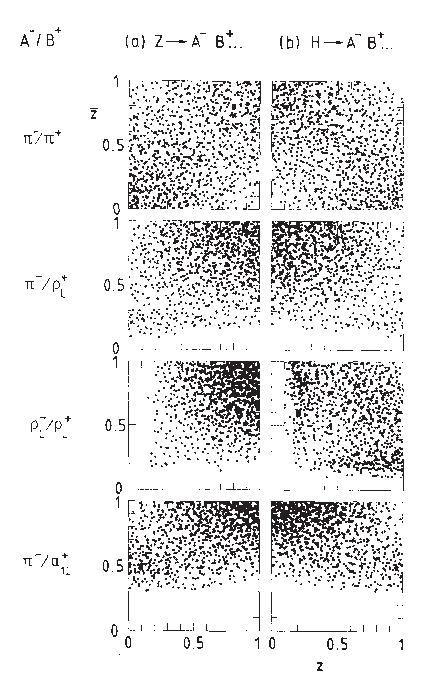
\includegraphics[width=.45\textwidth]{tau/theory}
\caption[An example of  difference in distributions for \HiggsToTauTau and \ZToTauTau.]
{
The two-dimensional distribution of (a) \HepProcess{\PZ \to \APtauon \Ptauon \to A^- B^+ \Pnut \APnut } (b) \HepProcess{\PHiggs \to \APtauon \Ptauon \to A^- B^+ \Pnut \APnut } events shown as functions of the energy fractions of $z = E_{A} / E_{\Ptauon}$ and $\overline{z} =  E_{B} / E_{\APtauon}$. In descending order the four sets of plots are for the (\APtauon, \Ptauon) pair decaying into (\Ppiminus, \Ppiplus), (\Ppiminus, $\rho_L^+$), ($\rho_L^-$, $\rho_L^+$) and finally (\Ppiminus, $a_{1L}^+$), each together with a \Pnut \APnut neutrino-pair. Plot is taken from \cite{Bullock:1991my}.
}
\label{fig:tauTheorySpin}
\end{figure}
\end{comment}

The ability to identify tau decay mode is also a benchmark for detector performance. Since tau lepton has a very short life time \cite{Abreu:1991jn}, only its decay products can be detected via the tracking detectors and calorimeters. Therefore the performance of the calorimetric and track systems determines the ability to separate different tau decay modes.


The main difficulty in the classification is to classify 1-prong final states.  These final states involves \Ppizero, where two photons from \Ppizero decay could be poorly reconstructed. At high energy, \Ppizero is boosted making the reconstruction more challenging. The ability to reconstruct the two photons as separate entities requires good pattern recognition algorithm for photons and \ECAL spatial resolution. Hence the improved photon reconstruction in \Chapter{chap:Photon} is used in this study. The impact of the \ECAL transverse spatial resolution on the tau decay classification is demonstrated as well.


This chapter is organised in the following sections. Firstly, the analysis chain to identify tau decay modes will be described, followed by the \ECAL optimisation study using the decay mode classification as a benchmark. Lastly, the classification is further used in a proof-of-principle analysis to demonstrate the ability to identify \PHiggs from \PZ using  tau pair decay channel.

\section{Overview of the analysis}

The study of the tau final state classification in the context for the  \ECAL optimisation allows the analysis to discard reconstruction and detector issue that do not vary with the \ECAL design. For example, the early photon conversion that happens in the tracking detector would complicate the event topology. But since it is affected by the tracker design, it can be ignored in this analysis. \SECTION{sec:tauSim}  and \Section{sec:tauPreSel} discuss the pre-selection cuts to choose the signal samples and events for this analysis.

The classification is performed with a multivariate classifier. Discriminating variables are calculated before feeding into the classifier.  A multiclass classicisation is used to allow simultaneous classification between  multiple final states, described in \Section{}.

This classification is repeated for different energies of tau lepton decay to access the impact of energy on classification. The impact of the \ECAL design is studied afterwards, where the \ECAL square cell size is varied. An overall tau hadronic decay classification efficiency is constructed to allow direct and easy comparison between different detector design and different energies of the tau decay.

A proof-of-principle analysis to demonstrate the ability to identify \PHiggs from \PZ using  tau pair decay channel is presented in the \Section{}. The difference in the spin of the boson reflects in the different spin correlation of the tau pair. By extracting the spin correlation, parent bosons can be separated.

The follow sections on the analysis use the a 50\,GeV tau lepton decaying sample, reconstructed with nominal the \ILD detector model.

\section{Decay modes}

Tau lepton decays into a numerous number of final states. To study the predominant effect of the tau lepton decays, decay modes with branching ratio above 1\% are studied. This results in seven tau lepton decay modes. Their branching ratios, along with decay mode and final states are  shown in \Table{tab:TauDecayMode}, which in total covers 92.58\,\% tau decay. The most difficult final states to separate are \decayRhoFinalStateShort and \decayAiPhotonFinalStateShort, where photons from boosted \Ppizero are very challenging to reconstruct correctly.

\begin{table}[htbp]\centering
\smallskip
\begin{tabular}{l l r}
\hline
\hline
Decay modes & Detectable final states & Branching ratio\\
\hline
\decayElectron   &  \decayElectronShort  & 17.83$\pm$0.04   \\
\decayMuon &	\decayMuonShort & 17.41$\pm$0.04  \\
\decayPion  &   \decayPionShort	& 10.83$\pm$0.06   \\
\decayRho   & \decayRhoFinalStateShort& 25.52$\pm$0.09 \\
\decayAi   & \decayAiPhotonFinalStateShort	& 9.30$\pm$0.11    \\
\decayAi  &	\decayAiPionFinalStateShort    & 8.99$\pm$0.06  \\
\decayThreePionPhoton  &	\decayThreePionPhotonShort    & 2.70$\pm$0.08  \\
\hline
\hline
\end{tabular}
\caption[Decay modes, detectable final state particles and branching ratios of the seven major \Pgtm decays.]
{Decay modes, detectable final state particles and branching ratios of the seven major \Pgtm decays, taken from \cite{Agashe:2014kda}. \Pgtp decays similarly to \Pgtm.}
\label{tab:TauDecayMode}
\end{table}

\section{Simulation and reconstruction}
\label{sec:tauSim}

\eeToTauTau channel is chosen to study the tau lepton decay mode classification, due to its the simplest channel for tau decay. The choice of the detector model for simulation is \ILD. The initial state radiation (ISR) and the beam induced background were not simulated, as they are not significant. These beam specific effects does not vary with the \ECAL design. Hence they are not simulated for the detector optimisation study. Another reason for not simulating ISR is that the energy of the tau lepton would not be a constant with the ISR contribution.

Two million events were reconstructed with  \ilcsoft version v01-17-07 \cite{Gaede:82475} and \pandora version 3 \cite{Marshall:2015rfa}, where the photon reconstruction is described in \Chapter{chap:Photon}.


\section{Event pre-selection}
\label{sec:tauPreSel}


Some events are very difficult or almost impossible to reconstruct correctly. This can happen if particles are in the forward beam pipe direction, where the forward calorimeters are not simulated due to computational limitations, or if particles carry too little energies to be more significant than noises. Another type of reconstruction failure is when a photon converts into an electron pair in the tracking systems. Instead of reconstructing as a photon, an electron pair is reconstructed, which  alters the event topology and decrease the classification efficiencies. One more issue is that for the \ILD detector model concept, the gap region between barrel part of the calorimeter and the end cap part causes a significant drop in the particle reconstruction efficiency. The \pandora particle reconstruction does not attempt to recover reconstruction in the gap region. These reconstruction and detector issues do not vary with change of the \ECAL design in the later optimisation study. Therefore, these un-reconstructible events are discarded at MC level from the analysis. The selection cuts are listed in \Table{tab:tauPreSel} and the selection efficiency of each cut is presented in \Table{tab:tauPreSelEff}.



\begin{table}[htbp]\centering
\smallskip
\begin{tabular}{l r}
\hline
\hline
Cuts & Values\\
\hline
No photon early conversion & - \\
Visible energy of decay products & $ E_{vis,MC} > 5\,GeV$ \\
Polar angle acceptance & $0.6 > \absOf{\theta_{Z,MC}} > 0.3$ or $1.57 > \absOf{\theta_{Z,MC}} > 0.8$ \\

\hline
\hline
\end{tabular}
\caption[Pre-selection cuts for tau lepton decay final state classification.]
{Pre-selection cuts for tau lepton decay final state classification.}
\label{tab:tauPreSel}
\end{table}

The reason for no photon early conversion in the tracker has been stated above. The polar angle acceptance requires the MC tau lepton travelling to barrel or endcap only. The visible energy cut requires there is enough energy deposited in the calorimeter to have a proper reconstruction.   The visible energy of the MC tau lepton decay product is defined as the energy of the MC tau minus the energy of the MC tau neutrino. These cuts use MC truth information. Discarded events do not participate in the subsequent reinstruction and analysis.


\begin{table}[htbp]\centering
\smallskip
\begin{tabular}{ l r r r}
\hline
\hline
Final state   & \multicolumn{1}{R{0.2\textwidth}}{No photon conversion} & \multicolumn{1}{R{0.2\textwidth}}{Visible energy acceptance} &\multicolumn{1}{R{0.2\textwidth}}{Polar angle acceptance} \\
\hline
\decayElectronShort& 100.0 & 84.7& 66.2\\
\decayMuonShort &100.0& 85.2&66.7\\
\decayPionShort &100.0& 88.3&60.9\\
\decayRhoFinalStateShort &77.1&76.9&61.9\\
\decayAiPhotonFinalStateShort &61.3&61.2&50.5\\
\decayAiPionFinalStateShort &100.0&100.0&78.0\\
\decayThreePionPhotonShort &77.0&77.0&61.8\\
\hline
\hline
\end{tabular}
\caption[MC level pre-selection cut efficiencies for tau lepton decay final state classification.]
{MC level pre-selection cut efficiencies for tau lepton decay final state classification in percentages. Cuts are presented in a ``flow'' fashion, where each column contains all the cuts in columns to its left.}
\label{tab:tauPreSelEff}
\end{table}

The no photon early conversion cuts only effective against final states with \Ppizero, as \Ppizero decays to a photon pair. For final states with one \Ppizero, about 77\% events survived. For final states with two \Ppizero, about 61\% events survived, which is roughly $0.77^2$. For the visible angle acceptance, final states with only one particle are affected the most, whilst final states with more than one particles typically have more visible energies. The polar angle acceptance efficiencies depend on the final states, as light final states are boosted and more likely in the forward region.



%An low visible energy event is discarded if the total energy of the tau lepton visible decay products is below 5\,GeV. Requirement of the tau decay in the barrel or the end cap part of the calorimeter is defined as the polar angle of the tau is $ 17.2\degree < |\theta_{Z}| < 34.4\degree$ or $ 45.8\degree < |\theta_{Z}| < 90\degree$.


\section{Select single tau decay}

The \eeToTauTau channel contains two tau leptons travelling in opposite directions. Since the tau decay final state separation is applicable to single tau, \PFOs in one event are divided into two collections, each corresponding to one tau. Separation of \PFOs uses the principle thrust axis vector, explained in the \Section{sec:pandoraEvtShape}, which is the axis that most \PFOs aligned to. Two collections are obtained based on the sign of the scalar product between the thrust axis and the \PFO momentum vector. An example of the simulated \eeToTauTau event is shown in \Figure{fig:tauEvtDsp}.

\begin{figure}[tbph]
\centering
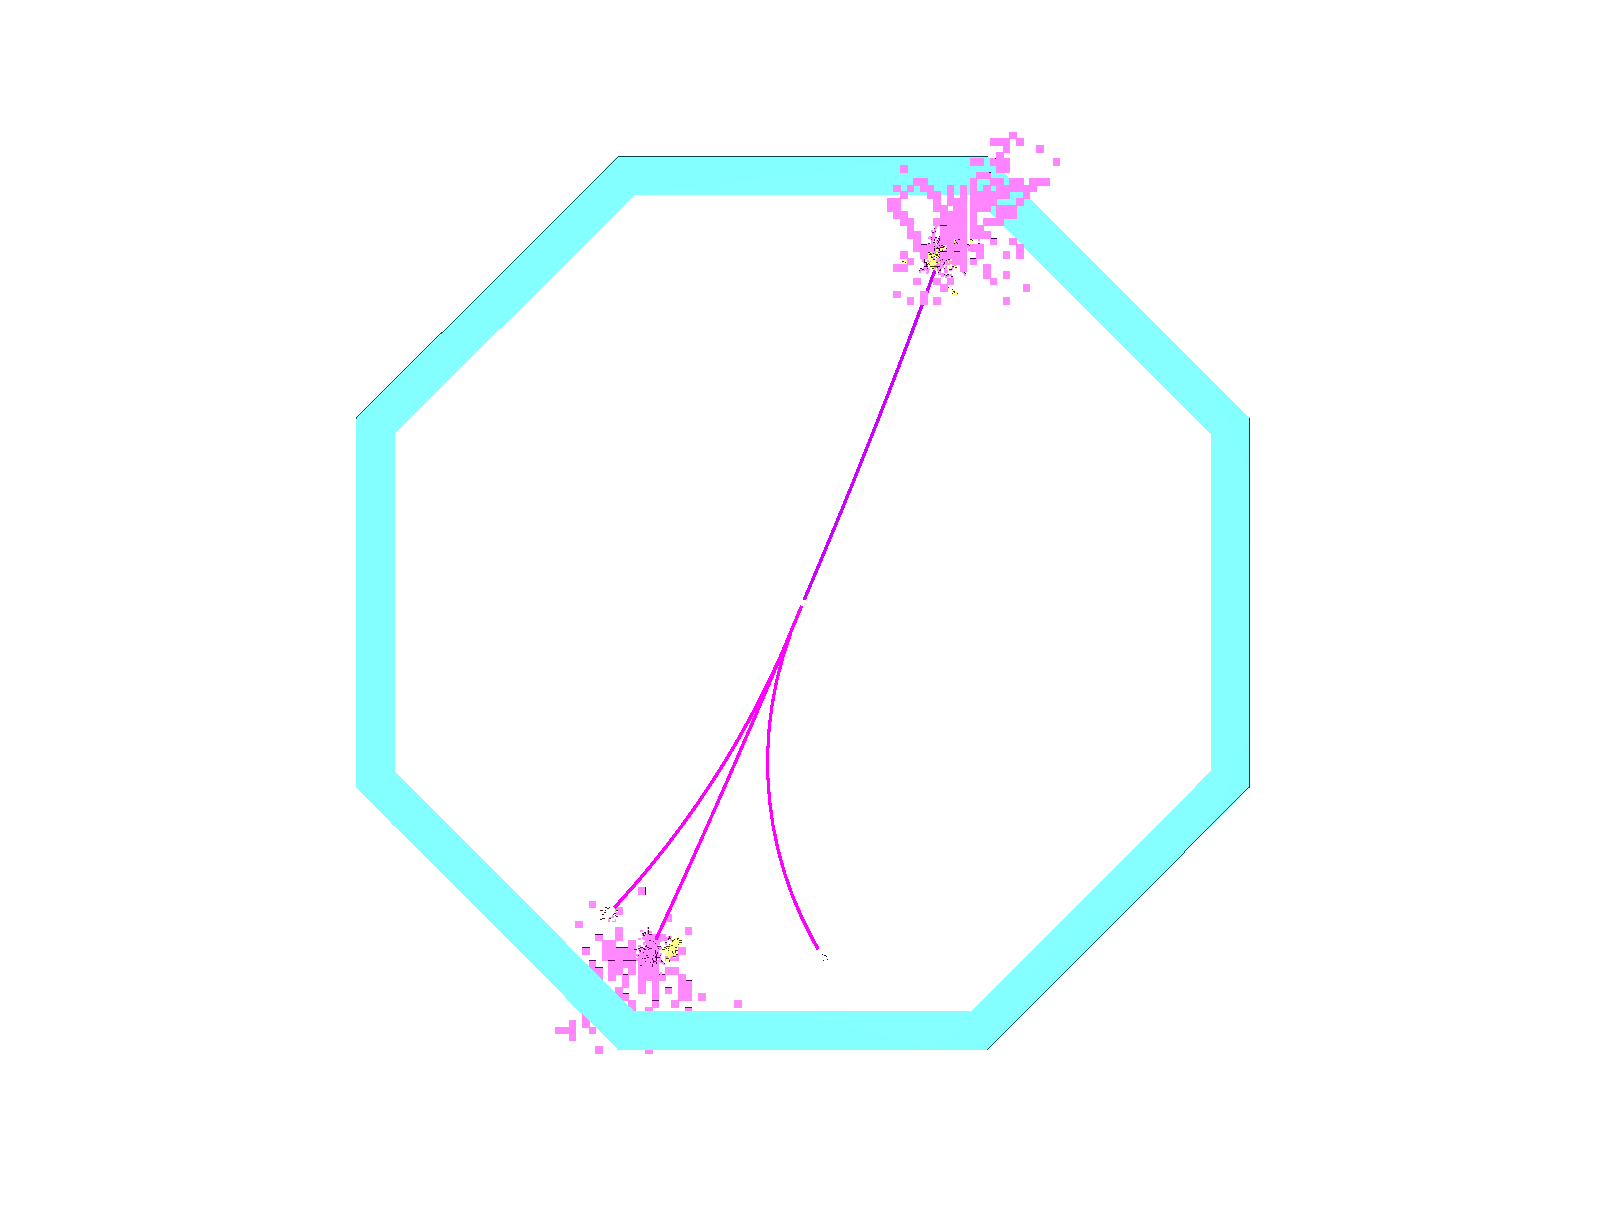
\includegraphics[width=0.45\textwidth]{tau/tau_evt_dsp2}
\caption{ An example event display of simulated \eeToTauTau event. The top tau decay is \decayRhoFinalStateShort final state and the bottom is \decayThreePionPhotonShort final state. Purple clusters are \Ppipm and yellow clusters are photons.  Blue region is the transverse cross section of the \ECAL barrel, looking along the beam line direction.}
\label{fig:tauEvtDsp}
\end{figure}



\section{Discriminative variables}

\begin{figure}[htbp]
\centering
% \begin{center}/\end{center} takes some additional vertical space
\begin{subfigure}[b]{0.45\textwidth}
 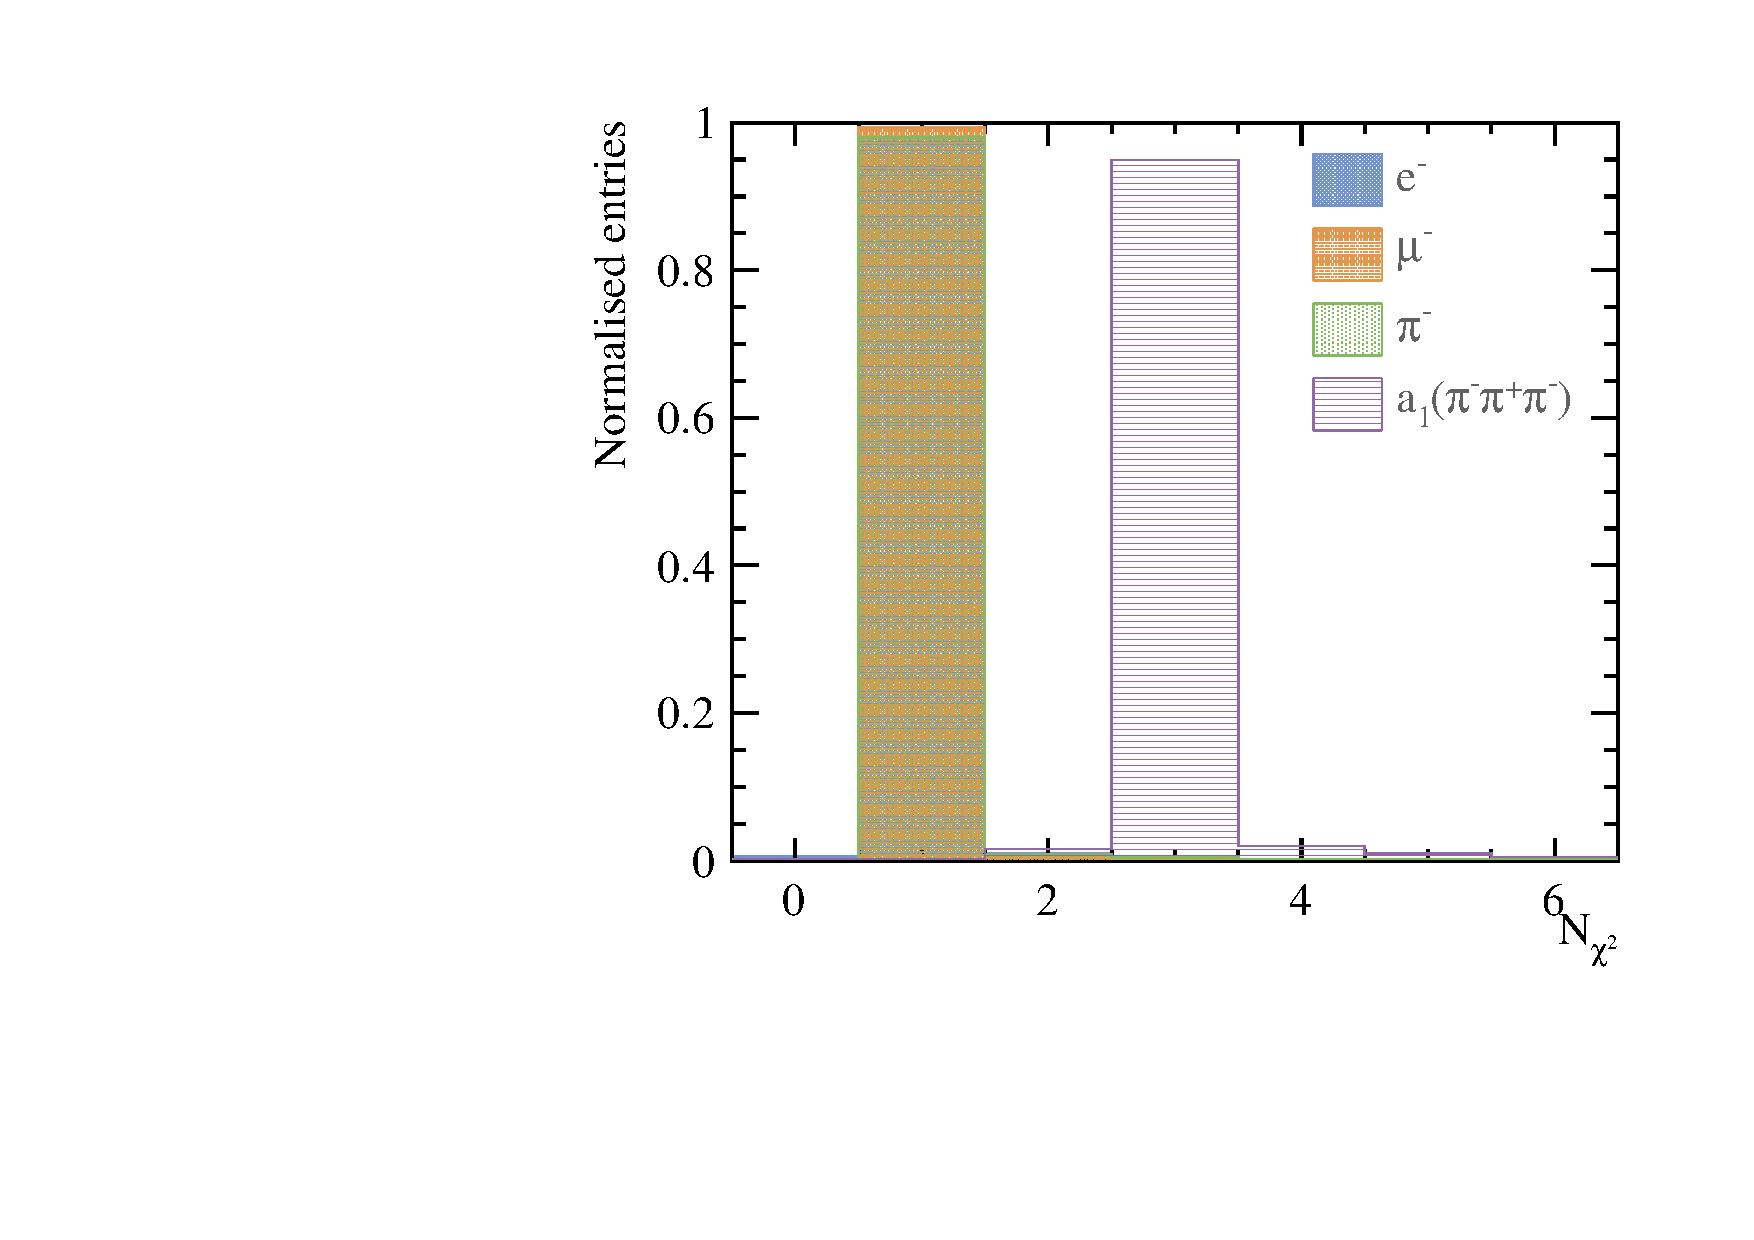
\includegraphics[width=\textwidth]{tau/var2/nCharge_100GeV_improved.pdf}
  \caption{}
  \label{fig:tauVarNCharge}
\end{subfigure}
\begin{subfigure}[b]{0.45\textwidth}
 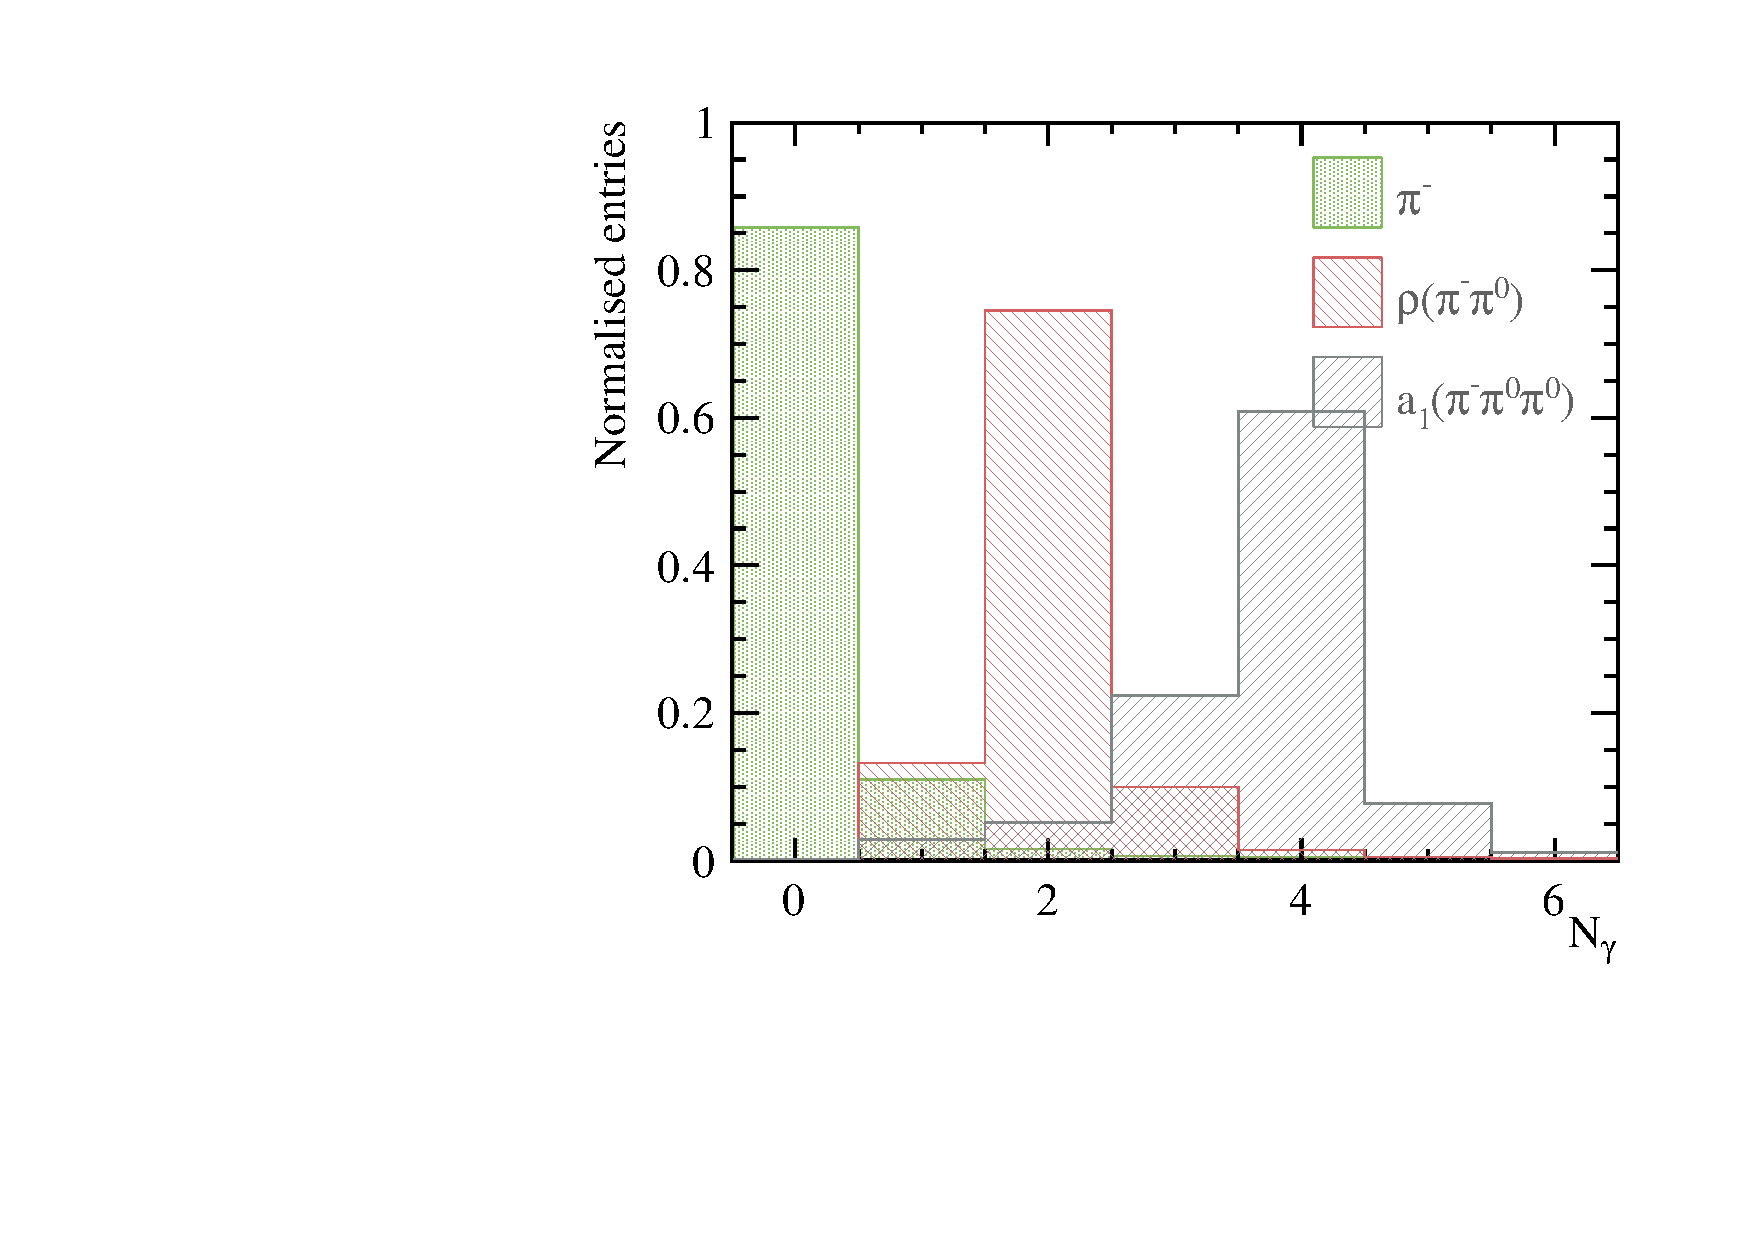
\includegraphics[width=\textwidth]{tau/var2/nPhoton_100GeV_improved.pdf}
  \caption{}
  \label{fig:tauVarNPhoton}
\end{subfigure}
\begin{subfigure}[b]{0.45\textwidth}
 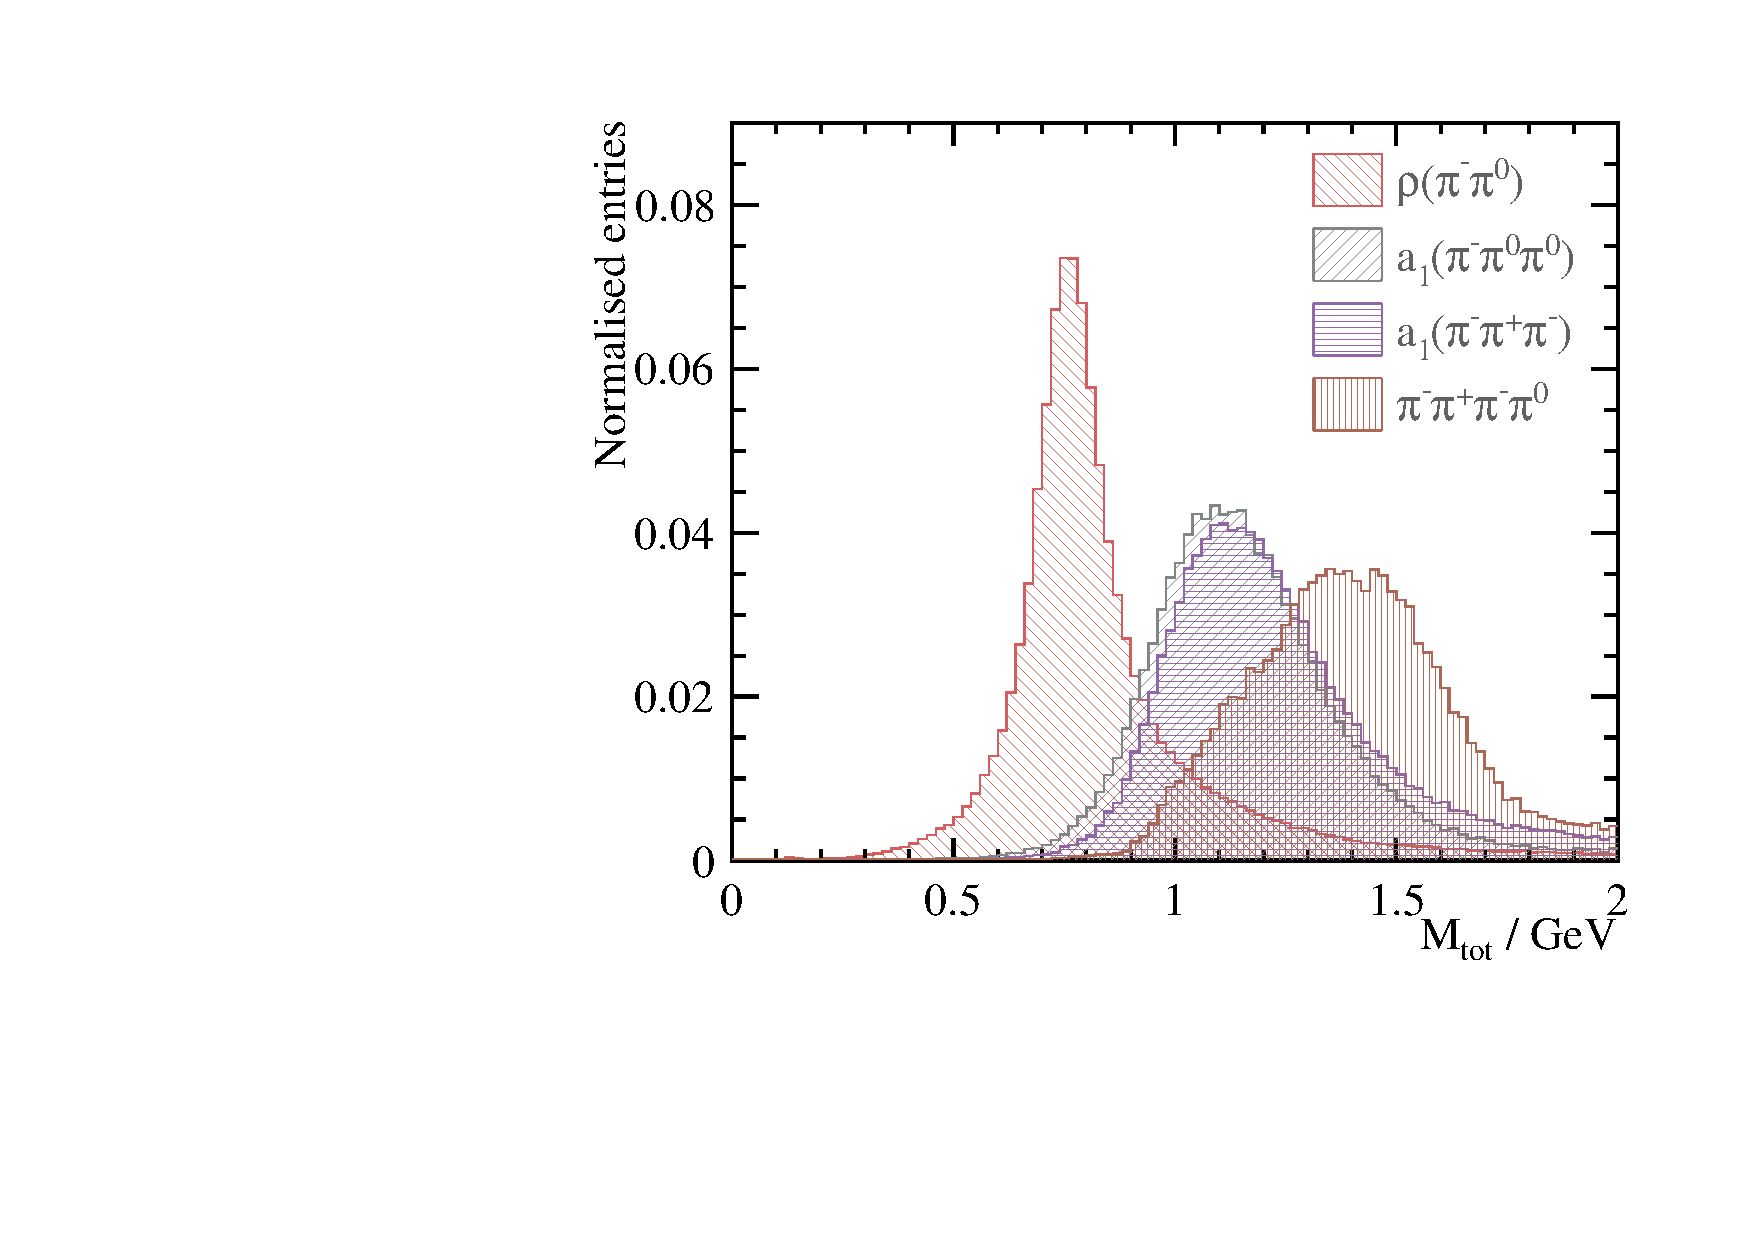
\includegraphics[width=\textwidth]{tau/var2/mVis_100GeV_improved_zoom.pdf}
  \caption{}
  \label{fig:tauVarMVis}
\end{subfigure}
\begin{subfigure}[b]{0.45\textwidth}
 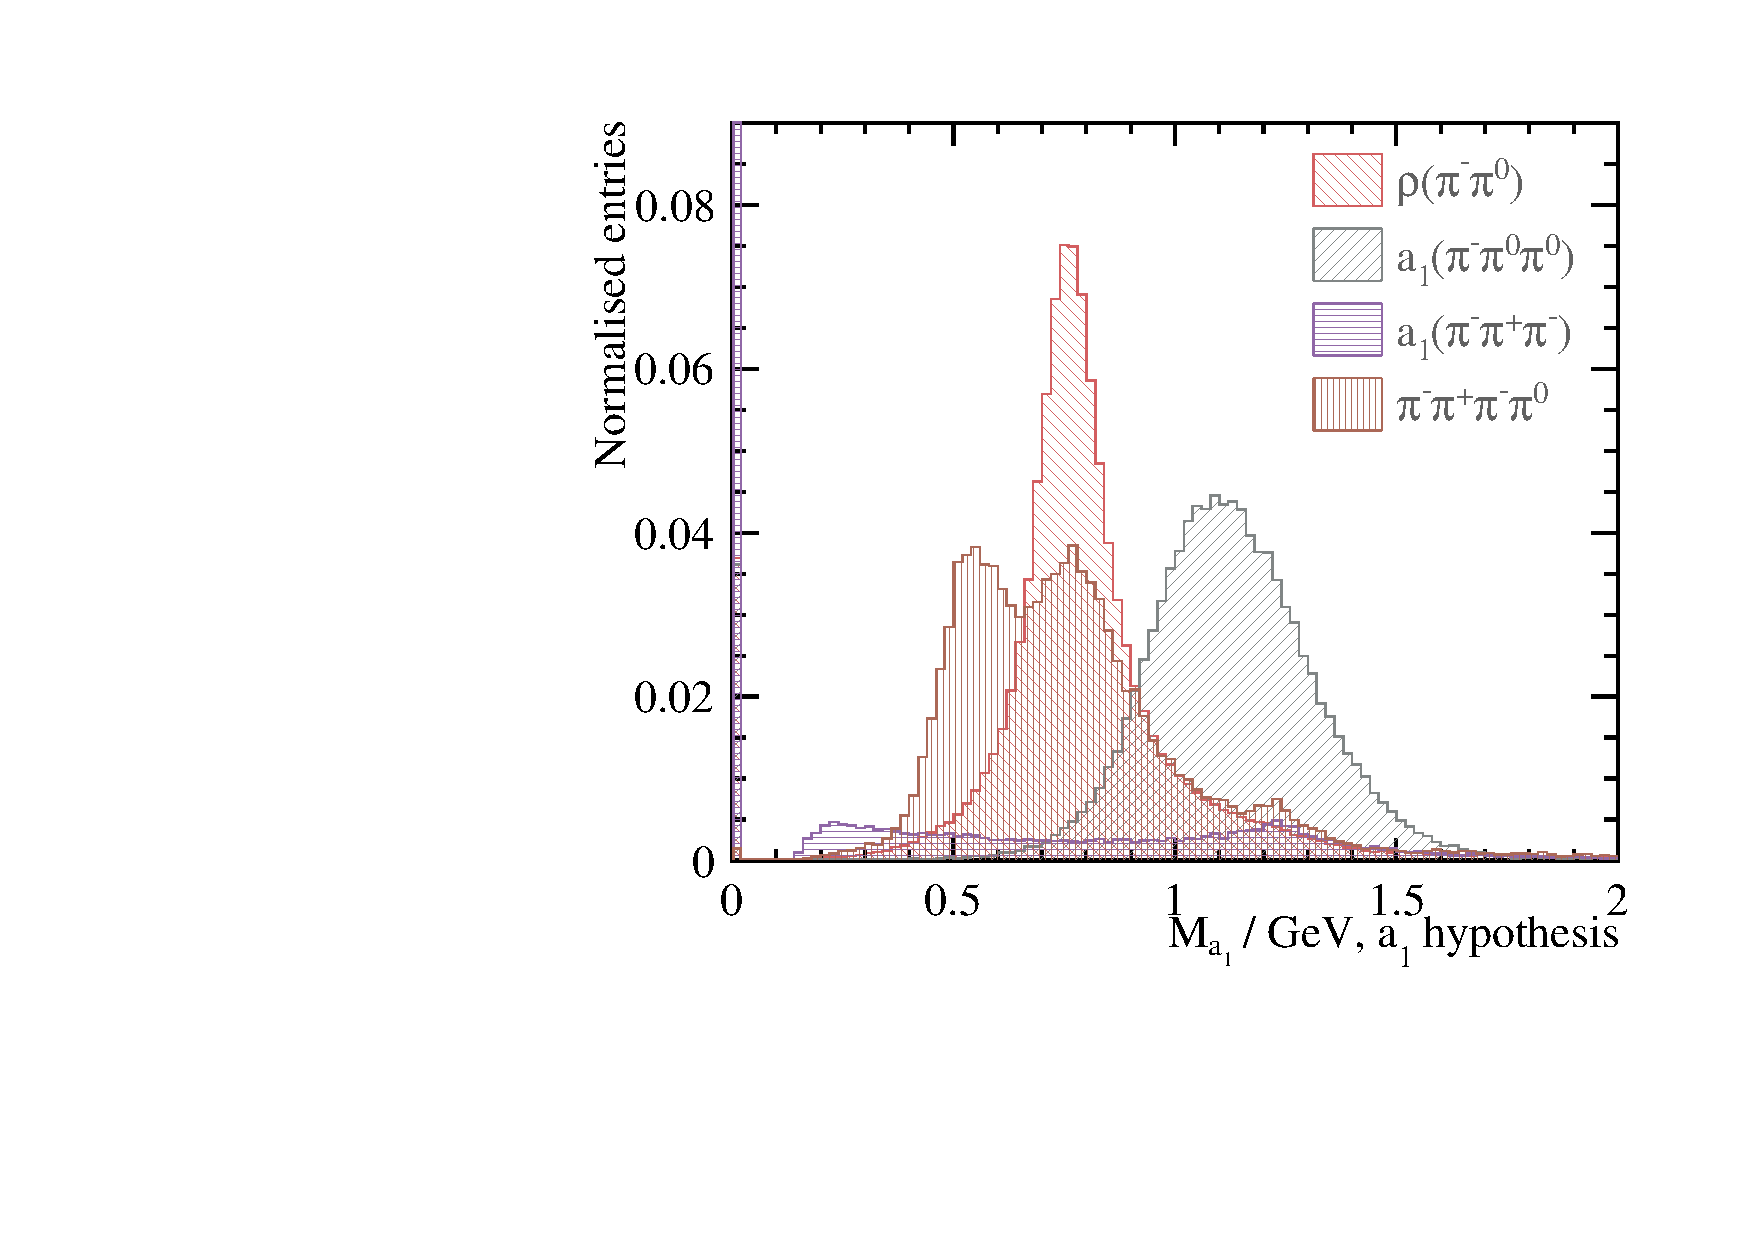
\includegraphics[width=\textwidth]{tau/var2/mA1A1Fit_100GeV_improved_zoom.pdf}
  \caption{}
  \label{fig:tauVarMA1}
\end{subfigure}

\caption
[Normalised distribution for selected variables.]
{
Normalised distribution for selected variables showing for seven final states, \decayElectronShort, \decayMuonShort, \decayPionShort, \decayRhoShort, \decayAiPhotonShort, \decayAiPionShort and \decayThreePionPhotonShort, separated using truth information. \FIGURE{fig:tauVarNCharge}, \Figure{fig:tauVarNPhoton}, \Figure{fig:tauVarMVis}, and \Figure{fig:tauVarMA1} show distributions for the number of tracks, the number of photons, the invariant mass of visible \PFOs, and the invariant mass of $a_1$ for \decayAiPhotonShort hypothesis test, respectively. The area for each final state is normalised to 1.
}
\label{fig:tauVar}
\end{figure}

Having pre-selected events, a set of discriminating variables are carefully developed the multivariate analysis (MVA). The full list of variables are shown in \Table{tab:tauVaraibles}.


\begin{table}[!htbp]\centering
\begin{tabular}{lr}
\hline
\hline
Category &  Variable \\
\hline
Invariant mass &  \multicolumn{1}{R{0.6\textwidth}}{$m_{vis}$, $m_{\charge}$, $m_\neutral$, $m_{\Pgg}$, $m_{\Pgpm}$} \\
Calorimetric info. &   \multicolumn{1}{R{0.6\textwidth}}{ $\% E_{\charge}$,  $\% E$ } \\
Energy & \multicolumn{1}{R{0.6\textwidth}}{ $\tilde{E}_{vis}$,  $\tilde{E}_{\charge}$, $\tilde{E}_{\Pmu}$, $\tilde{E}_{\Pe}$, $\tilde{E}_{\Pgg}$,  $\tilde{E}_{\Pgpm}$} \\
Number of \PFOs & \multicolumn{1}{R{0.6\textwidth}}{  ${N}_{\charge}$, ${N}_{\Pmu}$, ${N}_{\Pe}$, ${N}_{\Pgg}$,  ${N}_{\Pgpm}$} \\
\decayRhoShort reconstruction & \multicolumn{1}{R{0.6\textwidth}}{  $m_{\Pgpz}\parenths{\rho}$, $m_\rho$} \\
\decayAiPhotonShort reconstruction &  \multicolumn{1}{R{0.6\textwidth}}{  $m_{\Pgpz}\parenths{\Pai}$, $m^*_{\Pgpz}\parenths{\Pai}$, $m_{\Pai}$} \\
EM shower profile & $\delta{l}$, $t_0$, $\langle{w}\rangle$ \\
Calorimeter hit info. & $\bar{E}_{hit}$, $\%MIP$ \\
Track info. & $\Delta E/P$ \\
\hline
\hline
\end{tabular}
\caption
{Variables used in the MVA}
\label{tab:tauVaraibles}
\end{table}


These variables allow the multivariate classifier achieves a highly efficient tau decay mode classification. Different variables have discriminative powers against different final states. For convenience, variables are presented sequentially, although they participate the MVA simultaneously.



\begin{comment}
Having pre-selected samples, a set of discriminating variables was carefully developed to be used in the later multivariate analysis (MVA). These variables allow the multivariate classifier achieves a highly efficient tau decay mode classification. Different variables have discriminative powers against different final states. For convenience, variables are presented sequentially, although they participate the MVA simultaneously.

To differentiate 1-prong final states from 3-prong final states, number of tracks, shown in figure~\ref{fig:nCharge}, provides excellent separation power. Selection efficiencies are over 95\% for the 1-prong final states, and over 90\% for the 3-prong final states. For the 1-prong final states, they are further separated based on the number of photons reconstructed. Clear distinction between \decayPion, \decayRho and \decayAiPhoton decays mode can be seen in figure~\ref{fig:nPhoton}, where the overlap between any two decay modes is below 15\%. The two leptonic decay modes, \decayMuon and \decayElectron, have very different event topologies to other decay modes. For the \decayMuon decay mode, only muons deposit energies in the muon chamber. For the \decayElectron decay mode, electrons shower in the ECAL can be modelled by electromagnetic shower profiles. This information is used to distinguish a electron from a charged pion, including comparison of the observed and the expected electromagnetic shower profile, the matching between inner detector tracks and calorimeter clusters, and the fraction of calorimeter hits registered as minimum ionised particles.

\end{comment}

Some variables with most discriminative power are shown in figure~\ref{fig:nPfos}. In total 29 variables used in the multivariate analysis. The reason for the large number of variables is due to training seven decay modes at once, which will be discussed later.

Here is a full list of all variables used in the multivariate analysis. Energy of the \Pgt is assume to be the same as the energy of \Pepm colliding beam, which is half of the \rootS energy. Recoil momenta were calculated assuming the \Pem\Pep collision happened at the centre of mass energy. Both assumptions are largely valid when there is no ISR contribution.

\begin{itemize}
\item  $\frac{E_{ECal,HCal}}{E_{tot}}, charged$:  Sum of energy deposited in ECal and HCal, divided by the energy of charged particles
\item  $\frac{E_{ECal,HCal}}{E_{tot}}, all$:  	 Sum of energy deposited in ECal and HCal, divided by the energy of all particles
\item  $m_{vis}$:     	 Invariant mass of visible particles in GeV
\item  $\frac{E_{vis}}{E_{\Ptauon}}$:	 Sum of energy of all particles, divided by the energy of \Ptauon
\item  $\frac{E_{charged}}{E_{\Ptauon}}$:	 Sum of energy of charged particles, divided by the energy of \Ptauon
\item  $\frac{E_{\Pgmm}}{E_{\Ptauon}}$:	 Sum of energy of muons, divided by the energy of \Ptauon
\item  $\frac{E_{\Pem}}{E_{\Ptauon}}$:	 Sum of energy of electrons, divided by the energy of \Ptauon
\item  $\frac{E_{\Pgg}}{E_{\Ptauon}}$:	 Sum of energy of photons, divided by the energy of \Ptauon
\item  $\frac{E_{\Pgpm}}{E_{\Ptauon}}$:	 Sum of energy of charged pions, divided by the energy of \Ptauon
\item  $N_{charged}$:	 Number of charged particles
\item  $N_{\Pgmm}$:	 Number of muons
\item  $N_{\Pem}$:	 Number of electrons
\item  $N_{\Pgg}$:	 Number of photons
\item  $N_{\Pgpm}$:	 Number of charged pions
\item  $m_{\Pgg}$:     	 Invariant mass of photons in GeV
\item  $m_{charged}$:     	 Invariant mass of charged particles in GeV
\item  $m_{neutral}$:     	 Invariant mass of neutral particles in GeV
\item  $m_{\Pgpm}$:     	 Invariant mass of charged pions in GeV
\item  $m_{\Pgpz}, \decayRhoShort hypothesis$:     	 Fitted invariant mass of \Pgpz for \decayRhoShort hypothesis test
\item  $m_{\decayRhoShort}, \decayRhoShort hypothesis$:     	 Fitted invariant mass of \decayRhoShort for \decayRhoShort hypothesis test

\item  $m_{\Pgpz1}, \decayAiPhotonShort hypothesis$:     	 First fitted invariant mass of \Pgpz, for \decayAiPhotonShort hypothesis test, ordered by closeness to the true \Pgpz mass
\item  $m_{\Pgpz2}, \decayAiPhotonShort hypothesis$:     	 Second fitted invariant mass of \Pgpz, for \decayAiPhotonShort hypothesis test, ordered by closeness to the true \Pgpz mass
\item  $m_{\decayAiPhotonShort}, \decayAiPhotonShort hypothesis$:     	 Second fitted invariant mass of \decayAiPhotonShort, for \decayAiPhotonShort hypothesis test
\item  $\bar{E_{cell}}$:     	 Average energy deposited in a calorimeter cell in GeV
\item  $d_{trans,shower}$:    Transverse shower width for electromagnetic shower profile, averaged for all clusters in the ECal
\item  $l_{long,shower}$:    Longitudinal start layer for electromagnetic shower profile, averaged for all clusters in the ECal
\item  $\Delta{l_{long,shower}}$:    Longitudinal discrepancy for electromagnetic shower profile, averaged for all clusters in the ECal
\item  $\%MIP$:    Fraction of calorimeter hits registered as minimum ionised particles, averaged for all clusters in the ECal
\item  $\frac{E}{P}$:   Energy divided by momentum, averaged for all clusters in the ECal
\end{itemize}

Number of photons is an important variable for separating decay modes. This information is only available due to the excellent photon reconstruction. Shown in \Figure{fig:nPfos}, the majority of \decayMuon, \decayPion and \decayAiPion final states have zero photon reconstructed. The \decayElectron final state event have one photon reconstructed instead of zero, due to the FSR effect. \decayRho and \decayThreePionPhoton have nearly 80\% events with two reconstructed photons, whilst \decayAiPion have over 60\% events with four reconstructed photons. The loss is efficiency is due to the increasing difficulty to separate nearby photons.

The number of charged PFOs can clearly separate the leptonic and 1-prong final states, from the 3-prong final states, shown in \Figure{fig:nPfos}. The efficiency of leptonic final states are over 98\%.

The invariant mass of the visible PFOs shows clear differences between different final states. \decayRho, \decayAiPhoton and \decayAiPion distribution show clear resonance at \Prho and \Pai. \decayElectron, \decayMuon and \decayPion distribution show much smaller invariant mass and \decayThreePionPhoton shows a large invariant mass than \Pai. The \decayElectron final state has a long tail of invariant mass due to the extra photons from the FSR.

$\frac{E_{ECal,HCal}}{E_{tot}}, charged$ and $\frac{E_{ECal,HCal}}{E_{tot}}, all$ are both very effective at picking out leptonic decay modes.

For final states containing \Prho and \Pai resonance, it is useful to use minimisation test for right pairing of the resonance. We will use \decayAiPhotonShort as an example. \decayRhoShort is very similar.

The minimisation of \decayAiPhotonShort hypothesis states

\begin{equation}
\label{eq:a1}
\chi_{\Pai}^{2} = {\left(\frac{m_{\Pai,fit} -  m_{\Pai}}{\sigma_{\Pai}}\right)}^{2} + {\left(\frac{{m_{\Pgpz,fit}} -  m_{\Pgpz}}{\sigma_{\Pgpz}}\right)}^{2} + {\left(\frac{{m_{\Pgpz^*,fit}} -  m_{\Pgpz}}{\sigma_{\Pgpz}}\right)}^{2}  \,,
\end{equation}

where $m_{\Pgpz,fit}$ and $m_{\Pgpz^*,fit}$  are the invariant masses of all possible two photons combinations, $\sigma_{\Pai}$ and $\sigma_{\Pgpz}$ are the half width of the invariant mass distribution of reconstructed \Pai and \Pgpz using the truth information, and $m_{\Pai}$ and $m_{\Pgp}$ are the masses of \Pai and \Pgpz, taken from \cite{Agashe:2014kda}. If there are only two or three photons, the $\chi_{\Pai}^{2}$ expression will be reduced and not including $m_{\Pgpz^*,fit}$ term, assuming two photons are merged in the reconstruction. If there are fewer than two photons, the $\chi_{\Pai}^{2}$ expression would only contain $m_{\Pai,fit}$ term.

For the \decayRho final state, a similar $\chi_{\Pgri}^{2}$ test for \Pgri hypothesis is used to extract $m_{\Pgri,fit}$ and $m_{\Pgpz,fit}$ variables. $\chi_{\Pgri}^{2}$ is similar to $\chi_{\Pai}^{2}$ with \Pgri replacing \Pai and only one $m_{\Pgpz,fit}$ term.


\Figure{fig:nPfos} shows the $m_{\Pai,fit}$ where \decayRho, \decayAiPhoton  and \decayThreePionPhoton final states contribute to the \Pai resonance, although only \decayAiPhoton final has a real \Pai resonance. This is due to the structure of the  $\chi_{\Pai}^{2}$ minimisation function allowing final states with more than two photons and one \Pgppm to contribute.

Last six variables in the list help to differentiate an electron final state to that of a charged pion. A charged pion that starts showering early in the calorimeter could have a similar topology to an electromagnetic shower. Nevertheless, a good separation between the two can be achieved with the help of these variables.

\section{Multivariate Analysis}

For the multivariate analysis, the multiclass class of the TMVA package \cite{Therhaag:2009dp} was used to perform a multiclass classification, which trains the seven final states simultaneously. The multiclass class is an extension of the standard two-class signal-background classifier.

There are two ways for the training. "One v.s. one" is each class is trained against each other class. And the overall likelihood is normalised. The second way to train is called "one v.s. all", which is when each class is trained against all other classes.

Using a three-class example, A, B and C, "one v.s. one" scheme trains A against B, B against C, and C against A. Then the likelihood is normalised. "One v.s. all" would train A against B plus C, B against A plus C, and C against A plus B.

TMVA multiclass implementation uses "one v.s. all" scheme. For each final state, the multiclass classifier will train the final state as the signal against all other final states as the background. This process is repeated for each final state. The classifier output for a single event is a normalised response for each final state, where the sum is one. The response of each final state of a event can be treated as the likelihood. The event is classified into a particular final state if the final state has the highest classifier output response. The advantage of using the multiclass is that the correlation between different final states are accounted for and the classifier output are correctly adjusted for multiple final states, hence one event can only be classified into one final state. The issue with the multiclass is that discriminative variables for each final state need enter the training stage, resulting in a large number of variables.

Half of the randomly selected samples were used in the training process and the other half were used for testing.

The TMVA multiclass classifier used is boosted decision tree with gradient boosting (BDTG), as it was found to give for the best performance. The MVA classifier is trained and optimised to give the best overall separation across all final states. MVA will be discuss further in \Section{}

\section{Result}


\begin{table}[htbp]
\centering

\smallskip
\small
\begin{tabular}{| l | r | r | r | r | r | r | r |}
\hline
  Reco $\downarrow$ True $\to$  & \decayElectronShort & \decayMuonShort &\decayPionShort & \decayRhoShortest &\decayAiPhotonShortest &\decayAiPionShortest &\decayThreePionPhotonShort \\
\hline

\decayElectronShort  &\textbf{99.8}&-&0.9&1.1&0.8&-&-\\
\decayMuonShort   &-&\textbf{99.5}&0.5&-&-&-&-\\
\decayPionShort  &-&0.3&\textbf{93.2}&0.9&-&0.4&-\\
\decayRhoShortest&-&-&4.1&\textbf{93.0}&10.5&0.6&2.8\\
\decayAiPhotonShortest&-&-&-&4.3&\textbf{88.2}&-&1.0\\
\decayAiPionShortest&-&-&1.0&0.3&-&\textbf{96.6}&6.9\\
\decayThreePionPhotonShort&-&-&-&0.4&0.4&2.4&\textbf{89.3}\\

\hline
\end{tabular}

\caption[]%
{The percentage of reconstructed decay modes corresponds to underlying true decay modes, with \rootSGeV{100} for nominal \CLICILD detector model. Bold numbers show the correctly reconstructed percentages. Numbers less than 0.25\% are not shown. Statistical uncertainties are less than 0.25\%. Final states include \Pgngt, which is not shown.}
\label{tab:TauSelExample}
\end{table}


The reconstruction efficiencies for the seven final state of the tau decaying with c.o.m. energy of 100 \,GeV for the nominal CLIC\_ILD detector are shown in \Table{tab:TauSelExample}. The perfect reconstruction would result in only terms in the diagonal.

The unprecedented high classification rate has been achieved. The improvement of photon reconstruction described in \Section{} improved the ability to separate 1-prong final state. Most notably,  \Figure{} shows number of photons have a high correct reconstruction efficiency.

For leptonic decay, the selection efficiency is above 99.5\% as the tracking system have much better resolution than the calorimeter.

The \decayMuonShort final state has very clear topology, as muon deposits energy in the muon chamber. Therefore, there is little confusion with other final states.

\decayElectronShort final state is well separated, due to the specialised variables aimed to differentiate early hadronic shower to electromagnetic shower. However, there is still about 1\% confusion in one prong final state.

For one prong final states, \decayPionShort, \decayRhoShortest, and \decayAiPhotonShortest, the confusion is mainly due to the imperfect separation of nearby photons, originated form \Ppizero.


Similarly the confusion between 3-prong final state, \decayAiPionShortest, and \decayThreePionPhotonShort is caused by the inability to resolve photon pairs.

\section{Electromagnetic calorimeter  optimisaiton}

As discussed above, the tau decay mode separation is an benchmark test of detector performance. The ability to resolve photon pairs is crucial to separate different 1-prong states, and different 3-prong state. One of the main feature of calorimeter design affecting the photon resolution is the size of electromagnetic calorimeter (ECal) cell for the high granular calorimeter. The finer ECal cell size is, the better resolution of reconstructing individual photons.


The classification is being tested with the impact of different \sqrtS and different ECal square cell sizes. Around two million events were simulated at each \sqrtS = 100, 200, 500 and 1000\,GeV, with each different ECal square cell sizes of 3, 5, 7, 10, 15 and 20\,mm. Events were simulated and reconstructed in the same way as described above, with same selection applied. MVA classifier was trained individually for each \sqrtS and each ECal square cell size, with same set of discriminative variables.

\begin{figure}[htbp]
\centering % \begin{center}/\end{center} takes some additional vertical space
%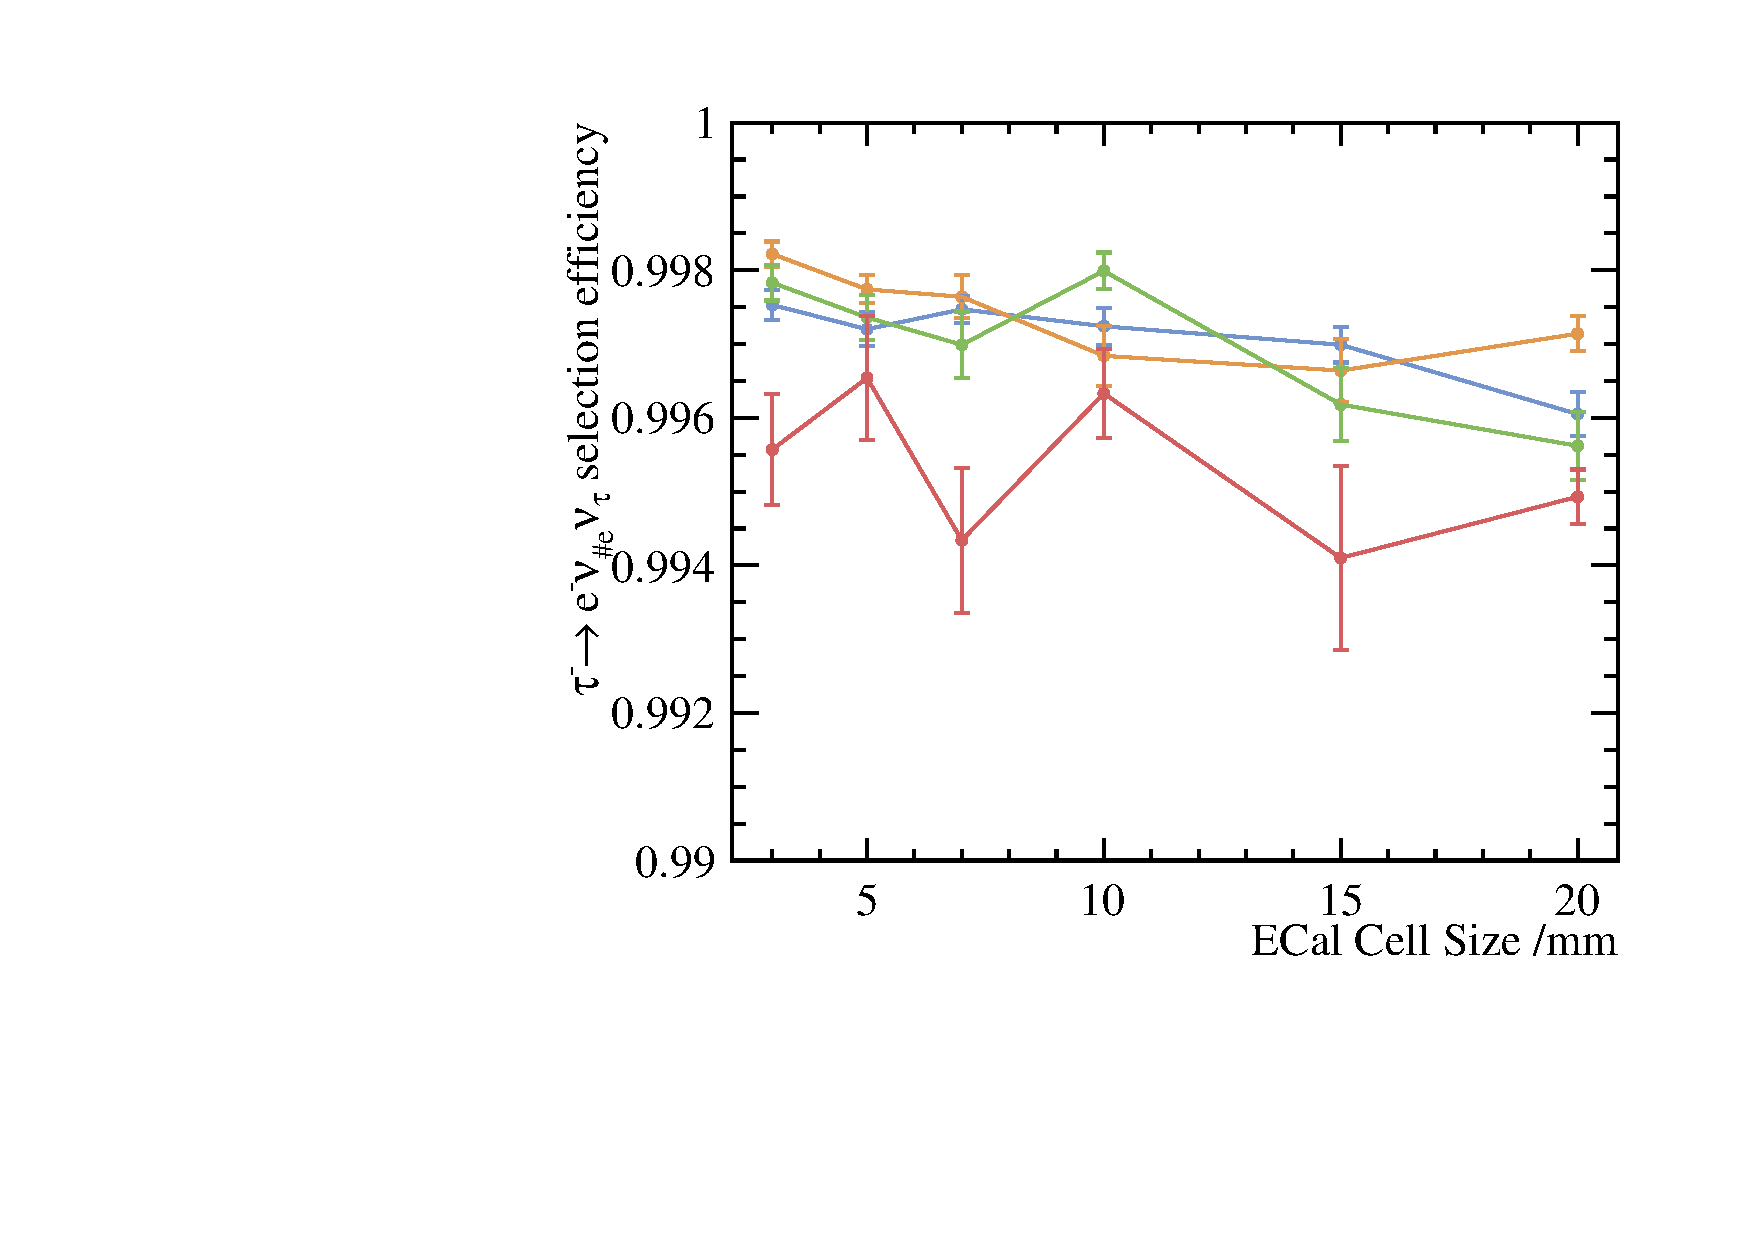
\includegraphics[width=.45\textwidth]{plots/decayMode0}
%\qquad
%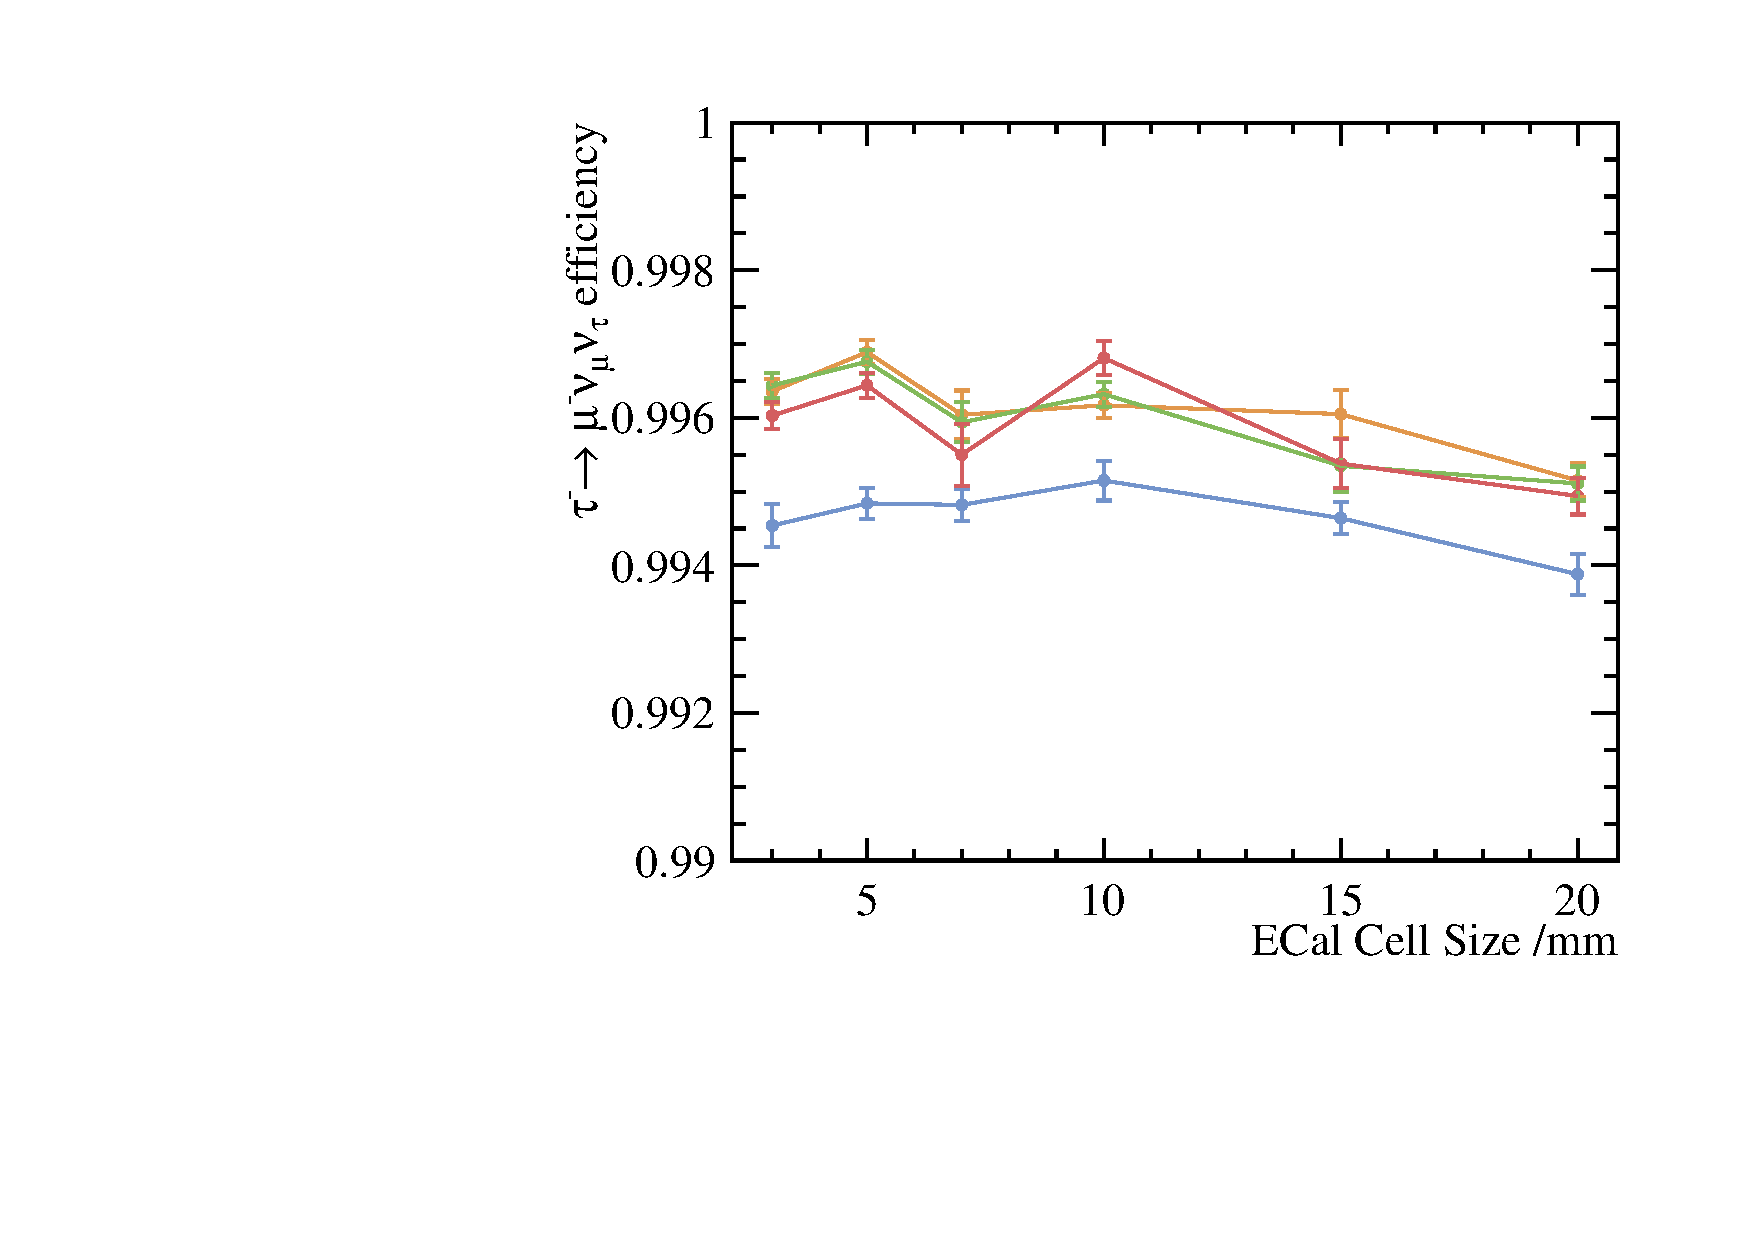
\includegraphics[width=.45\textwidth]{plots/decayMode1}
%\qquad
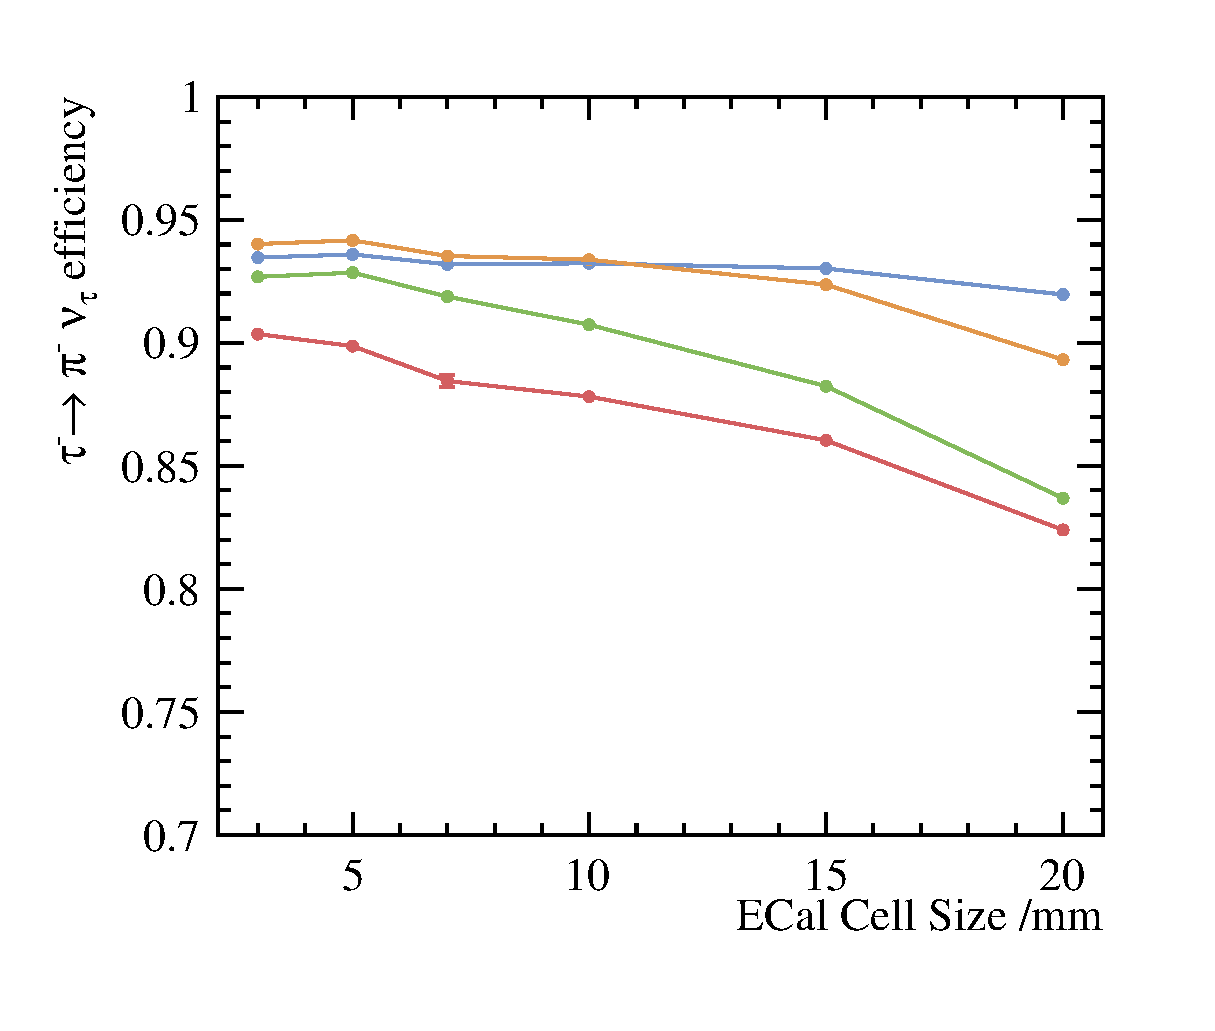
\includegraphics[width=.45\textwidth]{tau/decayMode2}
\qquad
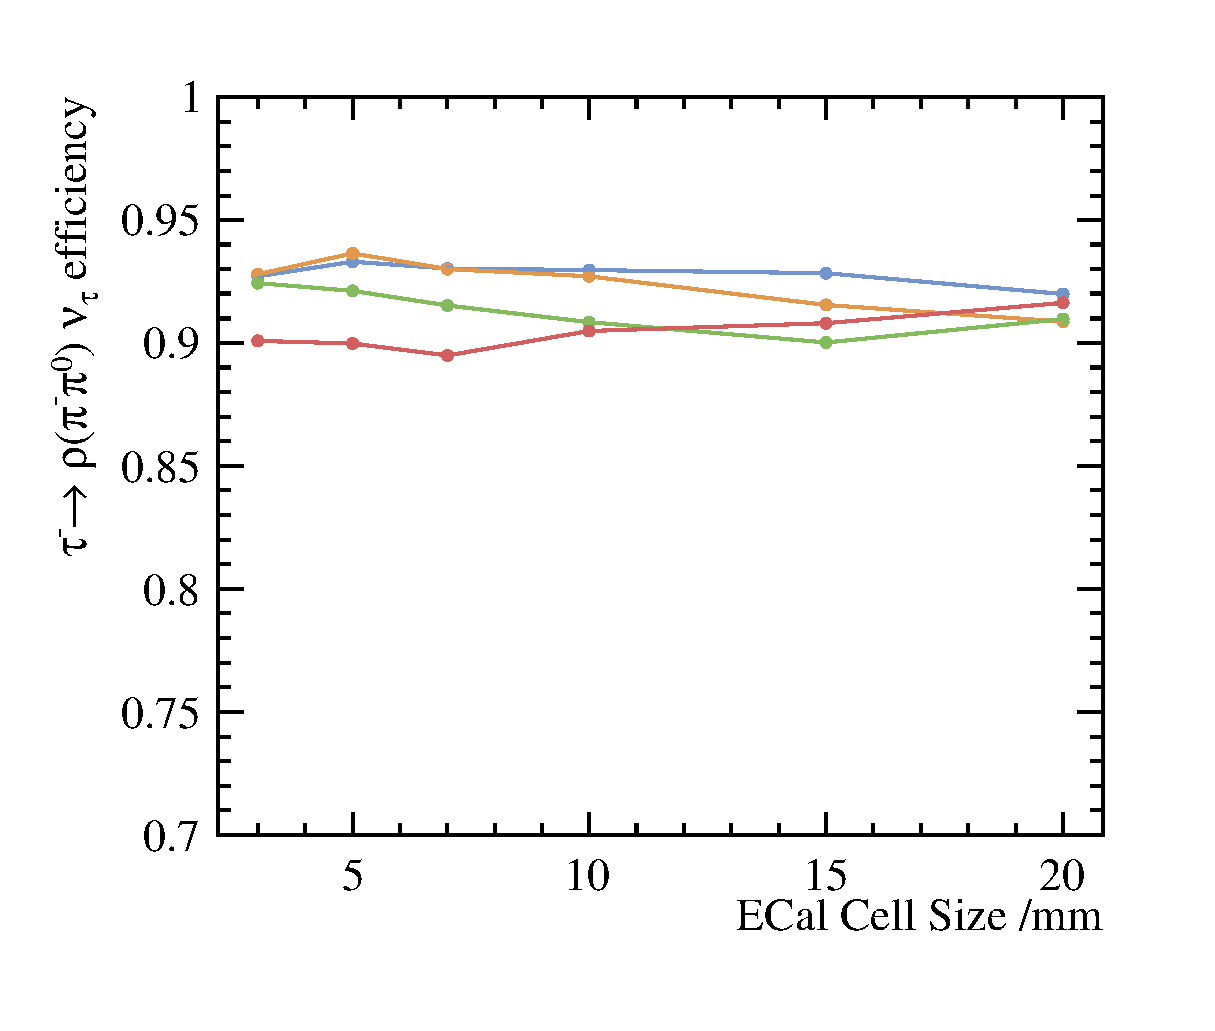
\includegraphics[width=.45\textwidth]{tau/decayMode3}
\qquad
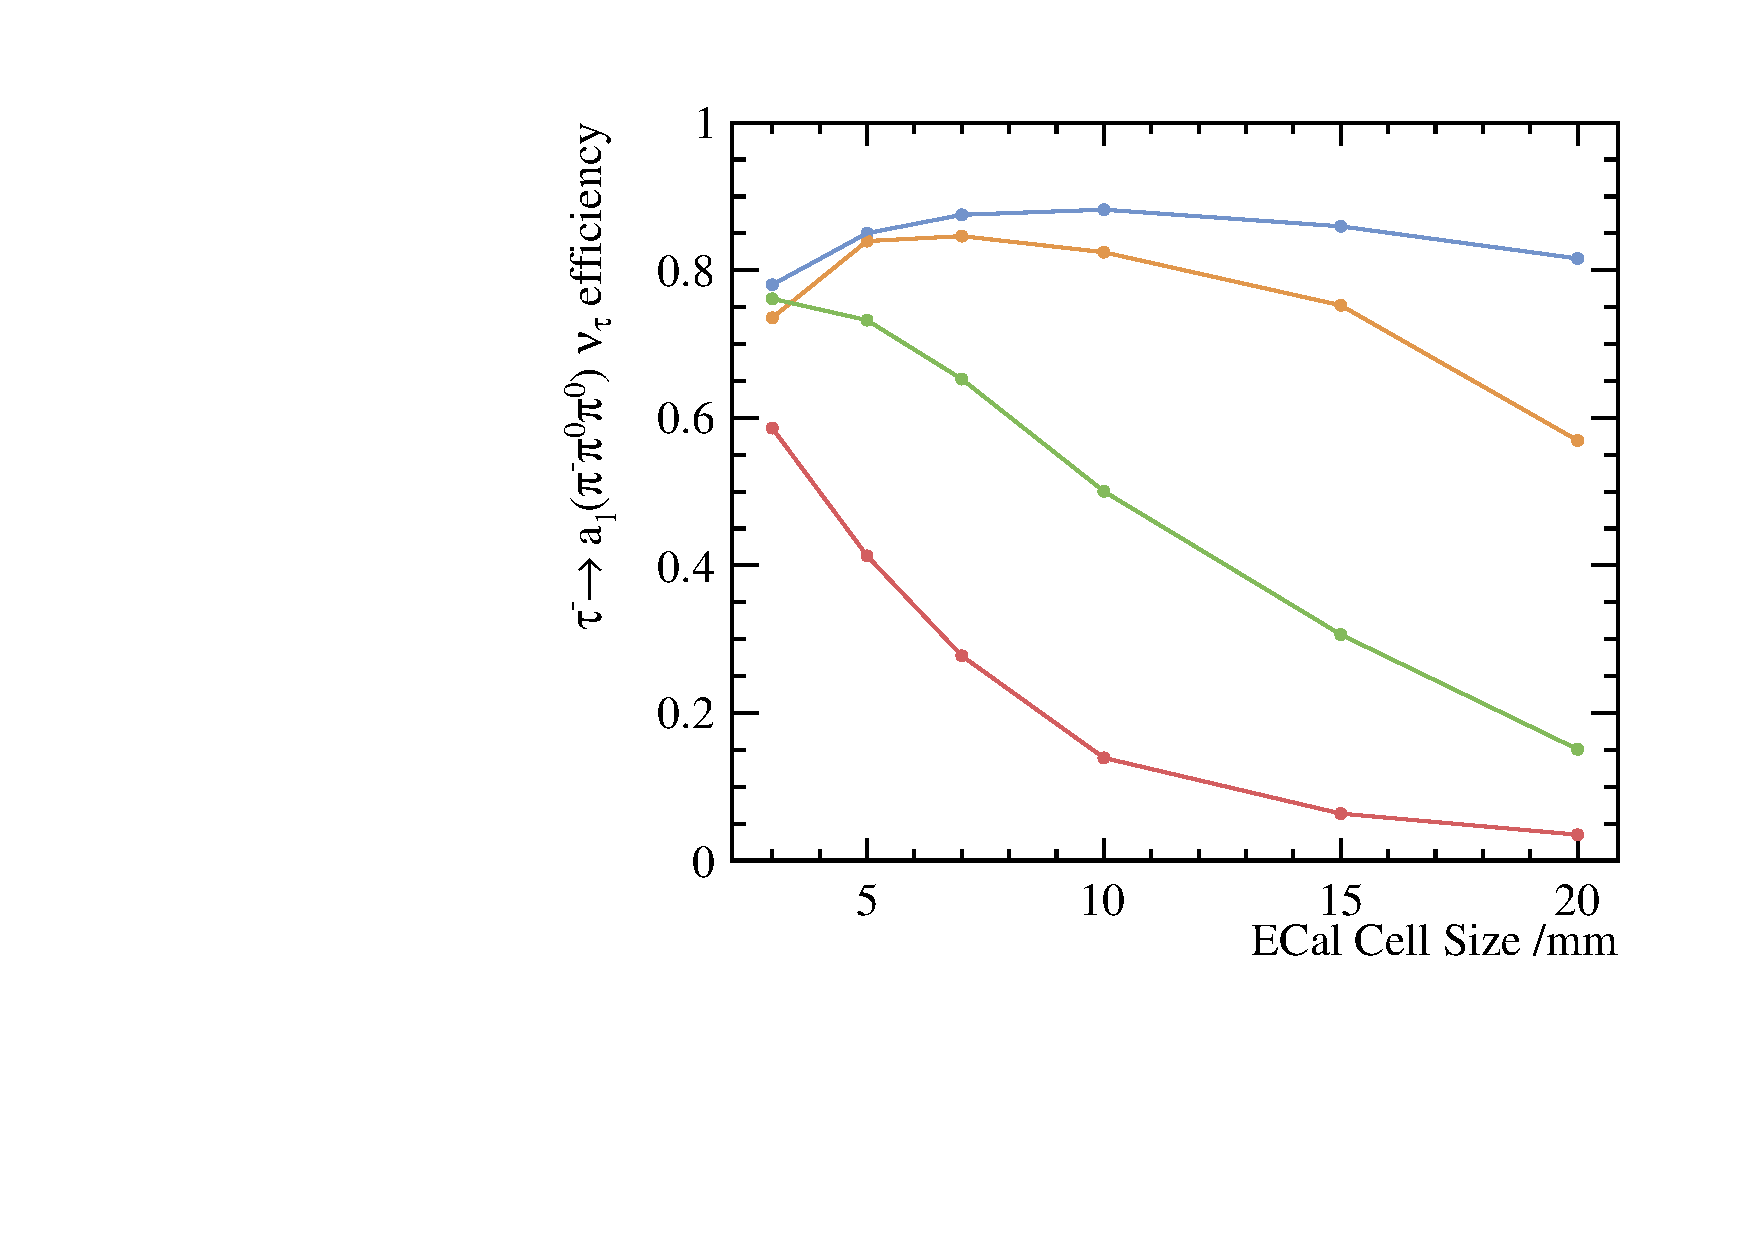
\includegraphics[width=.45\textwidth]{tau/decayMode4}
\qquad
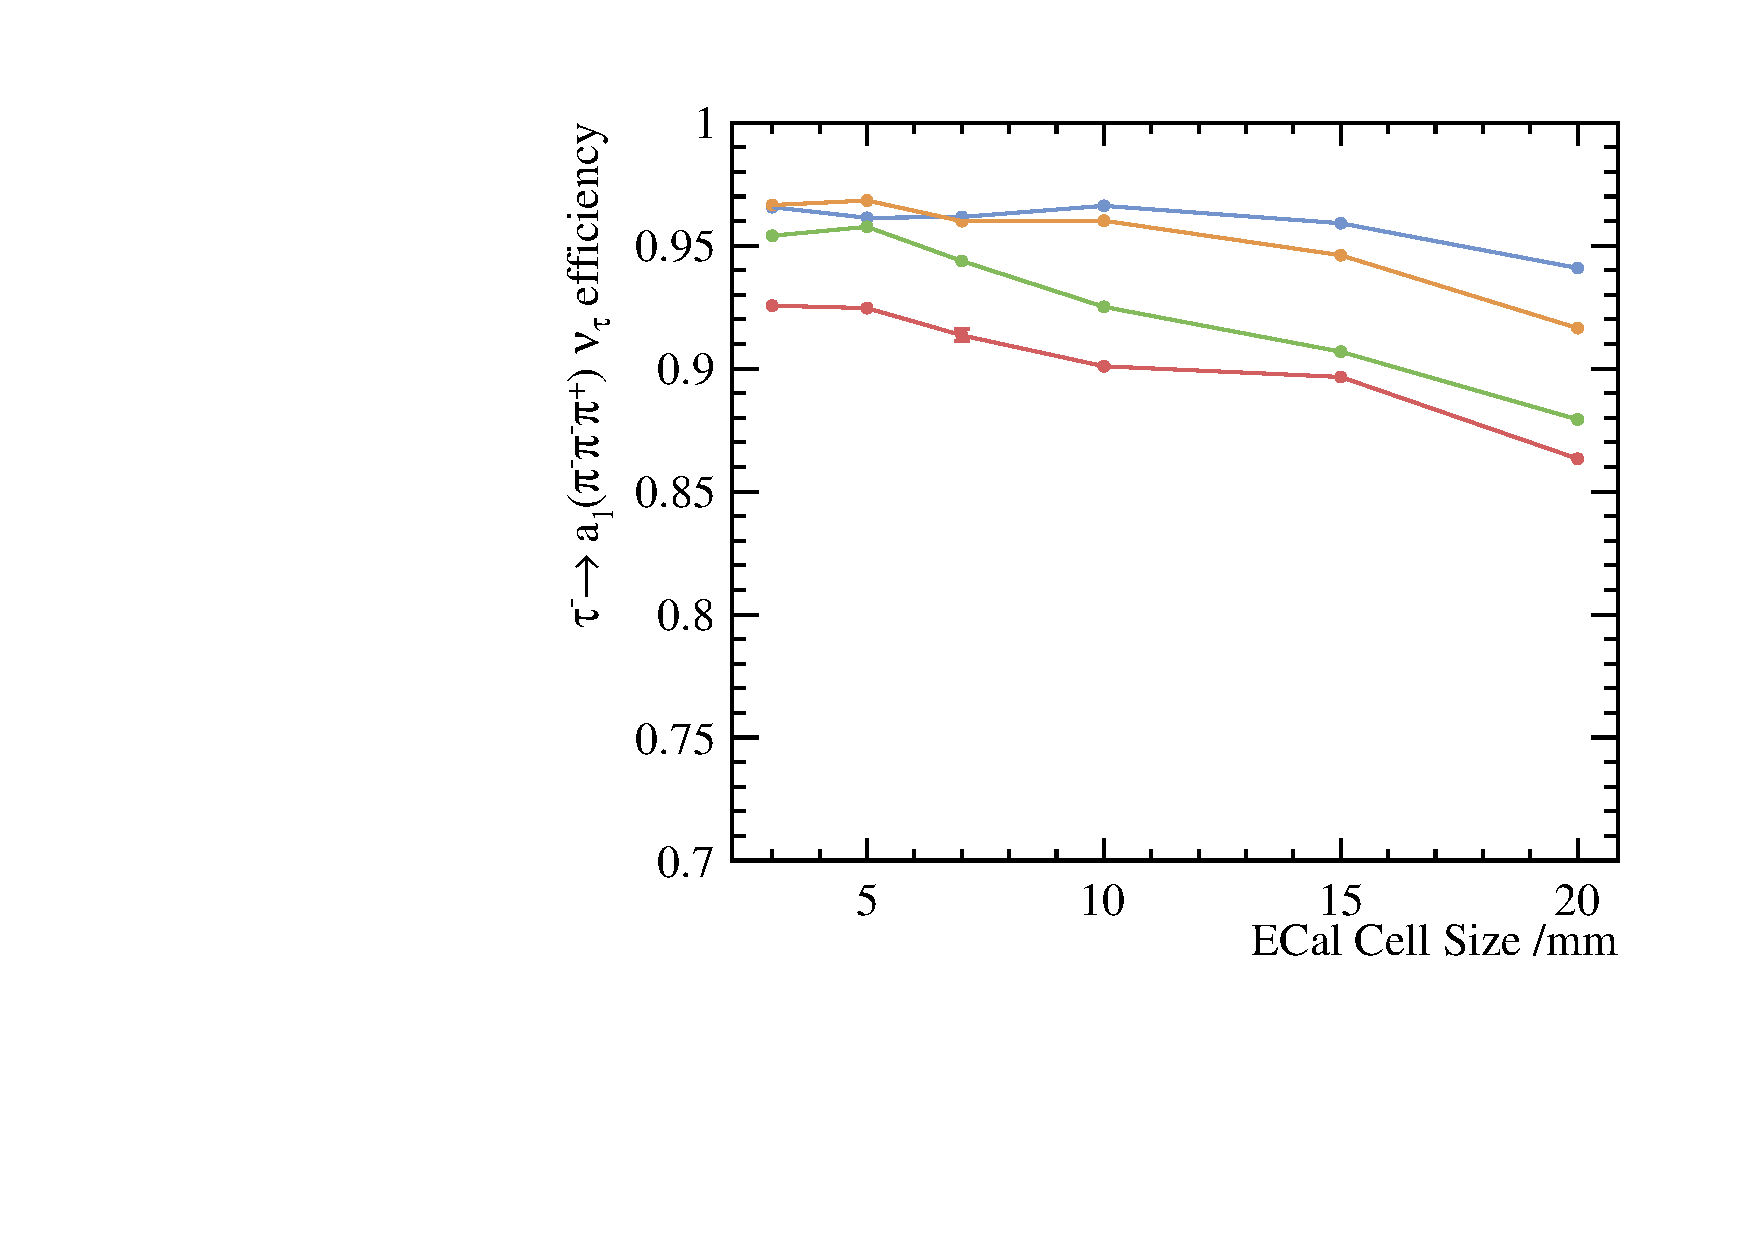
\includegraphics[width=.45\textwidth]{tau/decayMode5}
\qquad
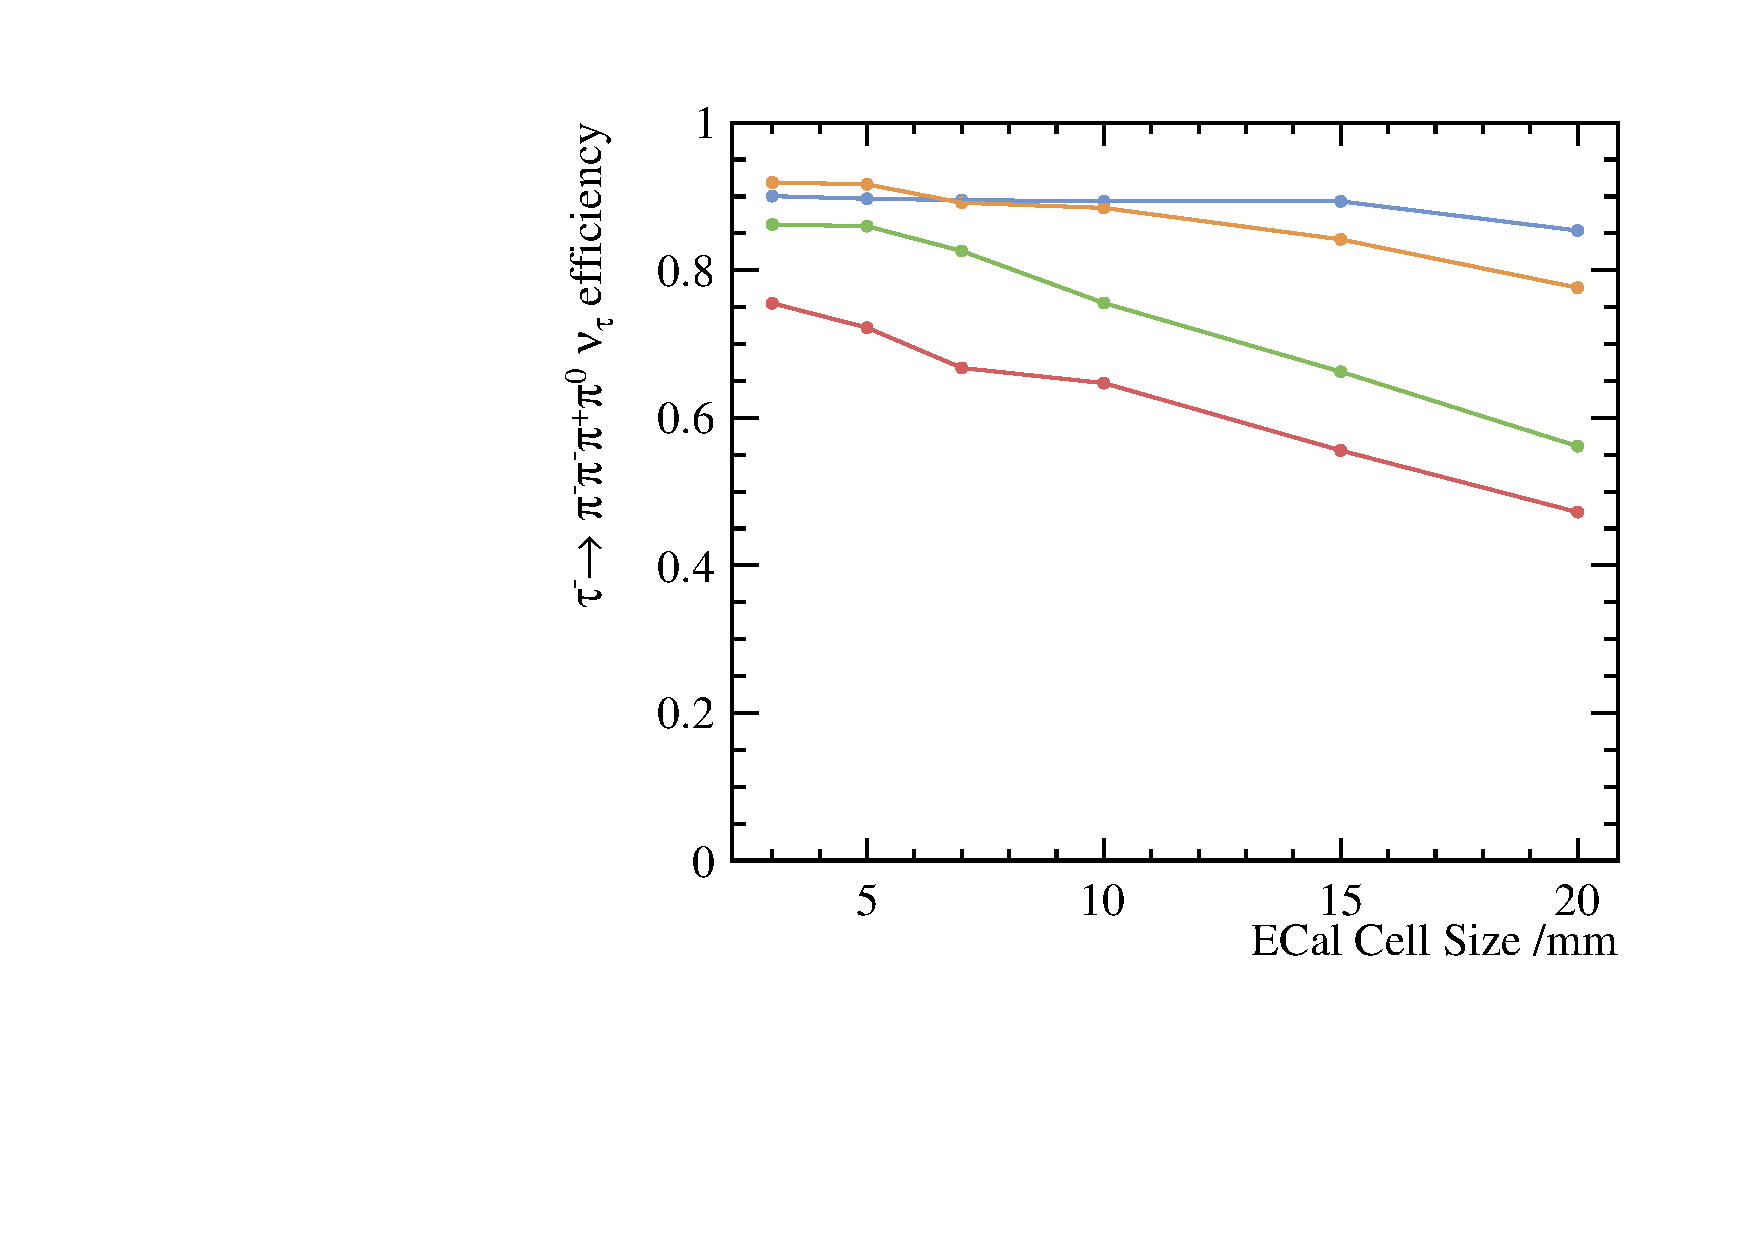
\includegraphics[width=.45\textwidth]{tau/decayMode6}
\qquad
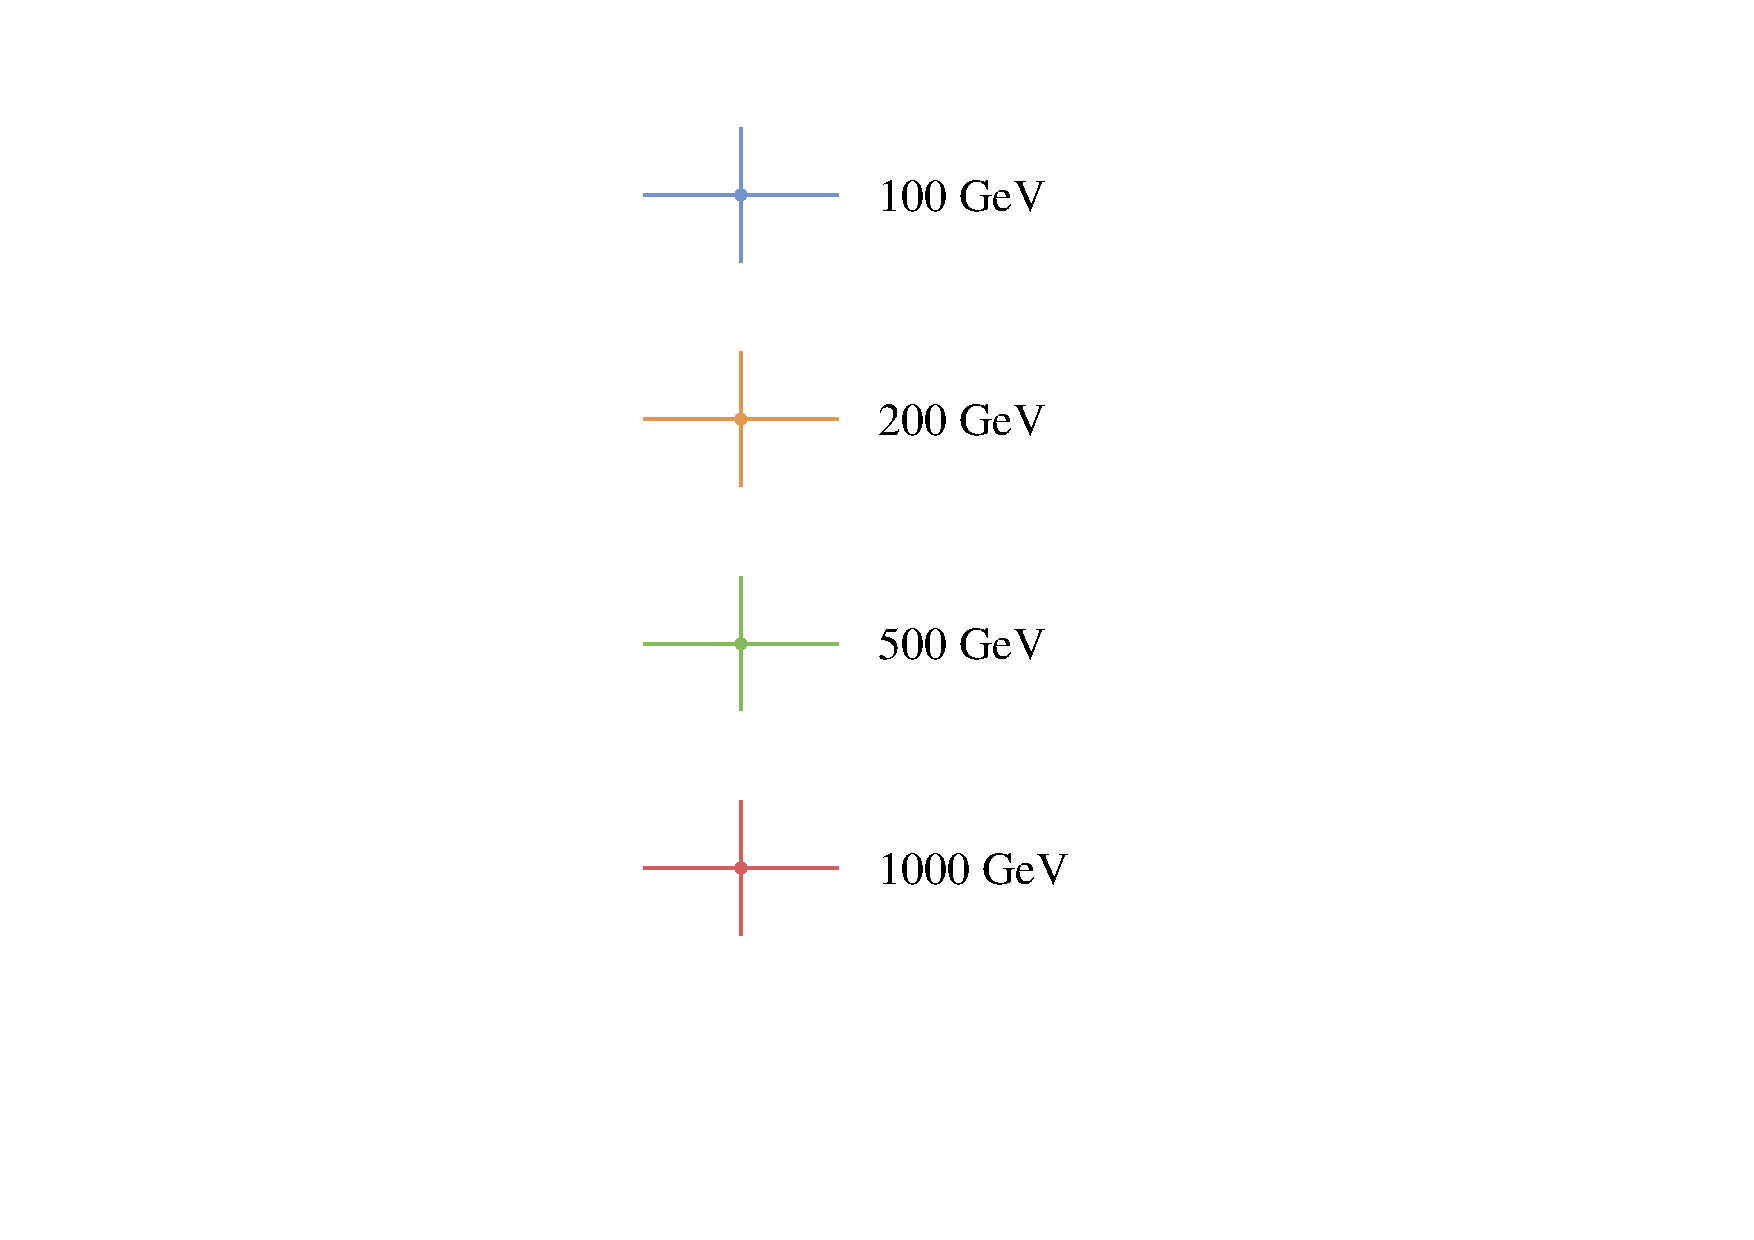
\includegraphics[width=.45\textwidth]{tau/legend}
%\qquad
%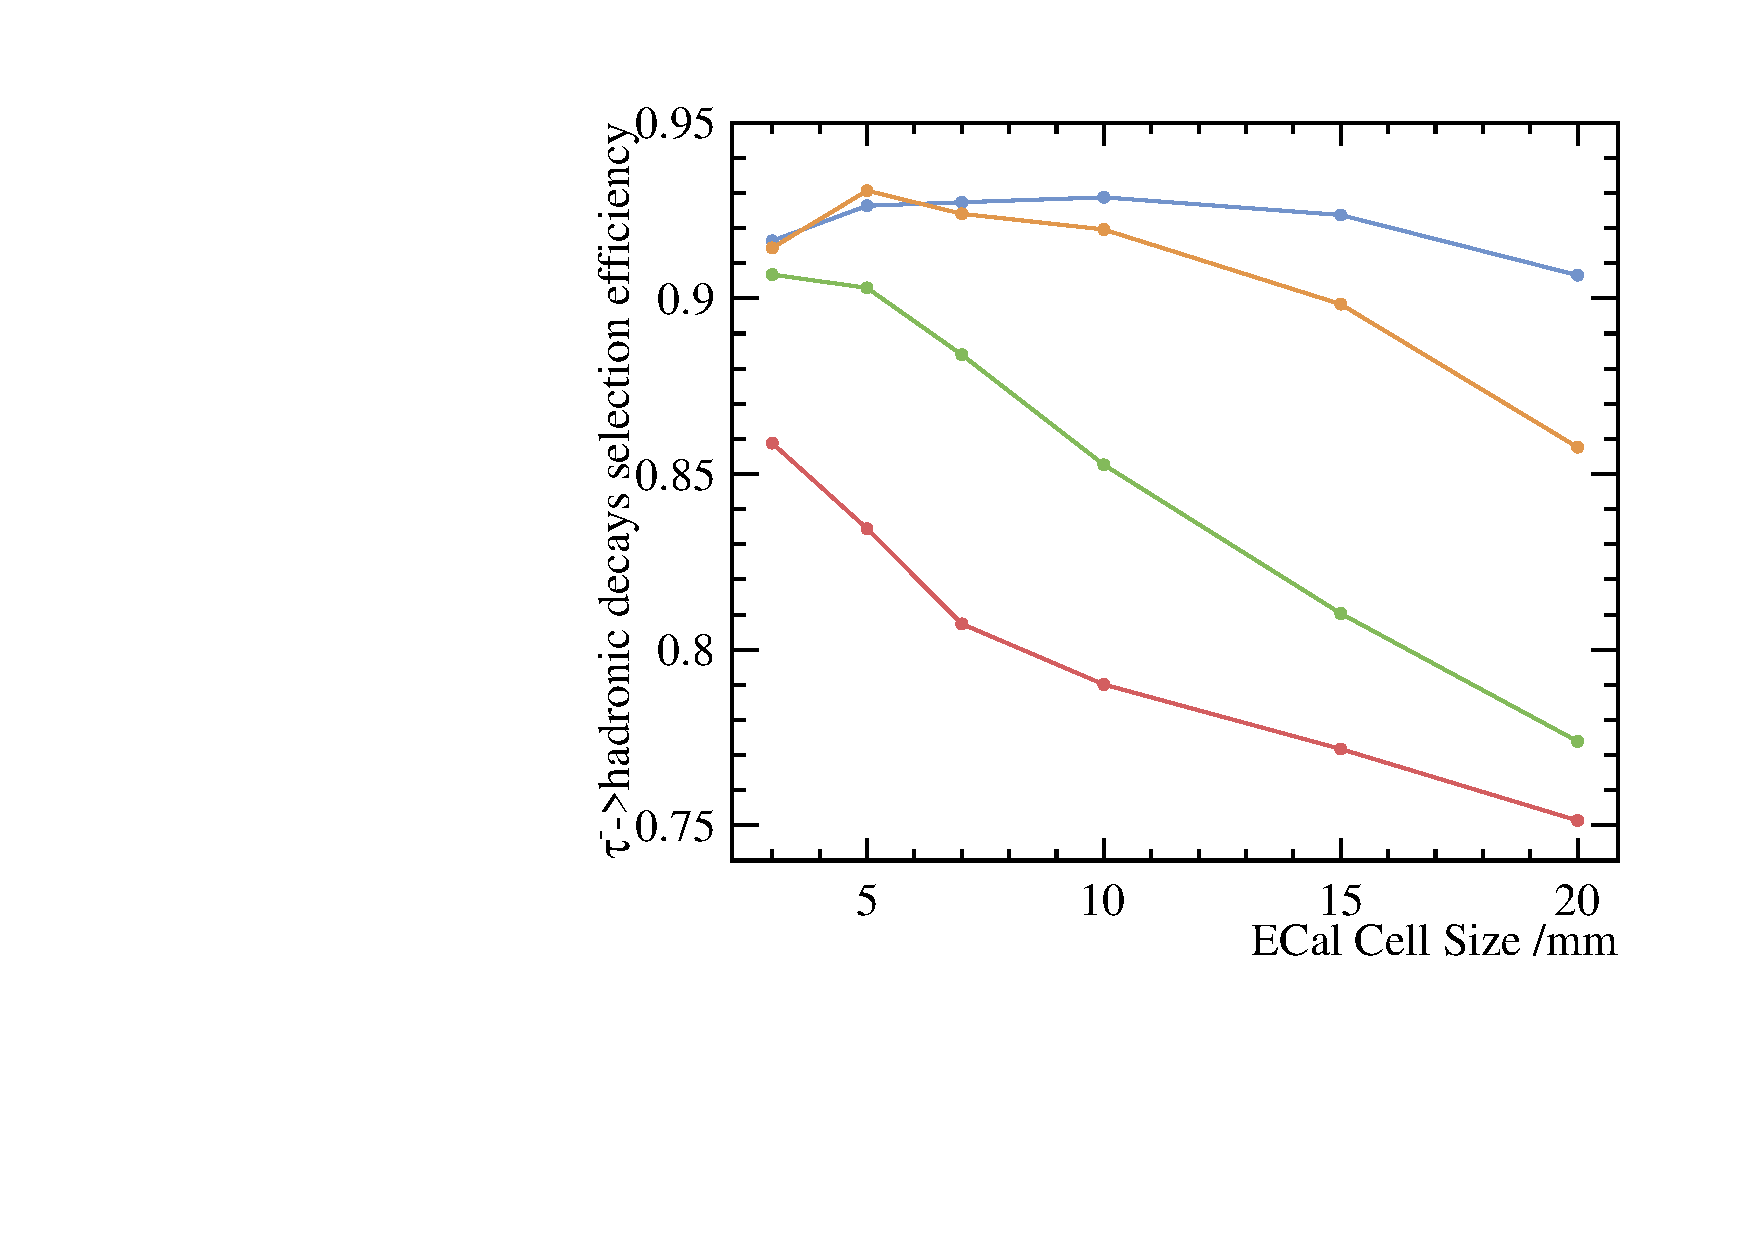
\includegraphics[width=.4\textwidth]{plots/hadEff}
% "\includegraphics" from the "graphicx" permits to crop (trim+clip)
% and rotate (angle) and image (and much more)
\caption[]%
{The selection efficiencies for various final states against the ECal cell size for different c.o.m. energies with the nominal \CLICILD detector model are shown. The top left, top right, middle left, middle right and bottom left plots are for the \decayPion, \decayRho,  \decayAiPhoton, \decayAiPion  and \decayThreePionPhoton  final states respectively. From the top to the bottom, blue, orange, green and red lines are representing the \sqrtS = 100, 200, 500 and 1000\,GeV respectively.}
\label{fig:TauPionEfficiency}
\end{figure}

To access the impact different ECal square size on detector performance, in particular ECal performance, the correct reconstruction efficiency for 1-prong and 3-prong final states is used as metric. The higher \sqrtS of the collision would degrade the performance, as photons are more boosted and more difficult to resolve.

The leptonic decay  correct reconstruction efficiency is not used as a metric as they are similar across different ECal cell sizes. This is because the \Pepm and \Pgmpm identifications mostly rely on the tracking system, which was not varied in this study. The energy deposited in the calorimeter are used for the association to the tracks but it has a small impact on the lepton identification.

\Figure{fig:TauPionEfficiency} shows that as the ECal cell sizes increase, the reconstruction efficiencies generally decrease. Larger cell sizes have lower spatial resolutions, making the separating of nearby photons more difficult.

For the \decayAiPhoton final state, the selection efficiency for 500\,GeV rises from ECal cell sizes 15\,mm to 20\,mm and the one for 1000\,GeV rises from 7\,, to 20\,mm actually goes up as cell size increases. This is because when the algorithm can not reconstruct four photons in the \decayAiPhoton final state, and the event topology would be very similar to the \decayRho final states.

For the \rootS = 100 and 200\,GeV, the selection efficiency of the 5\,mm ECal cell size is better than that of the 3\,mm. One possible explanation is that the  and the PandoraPFA have been optimised for the nominal ILD detector with the 5\,mm ECal cell size, which shares the same ECal structure with the nominal \CLICILD detector.


\begin{figure}[htbp]
\centering % \begin{center}/\end{center} takes some additional vertical space
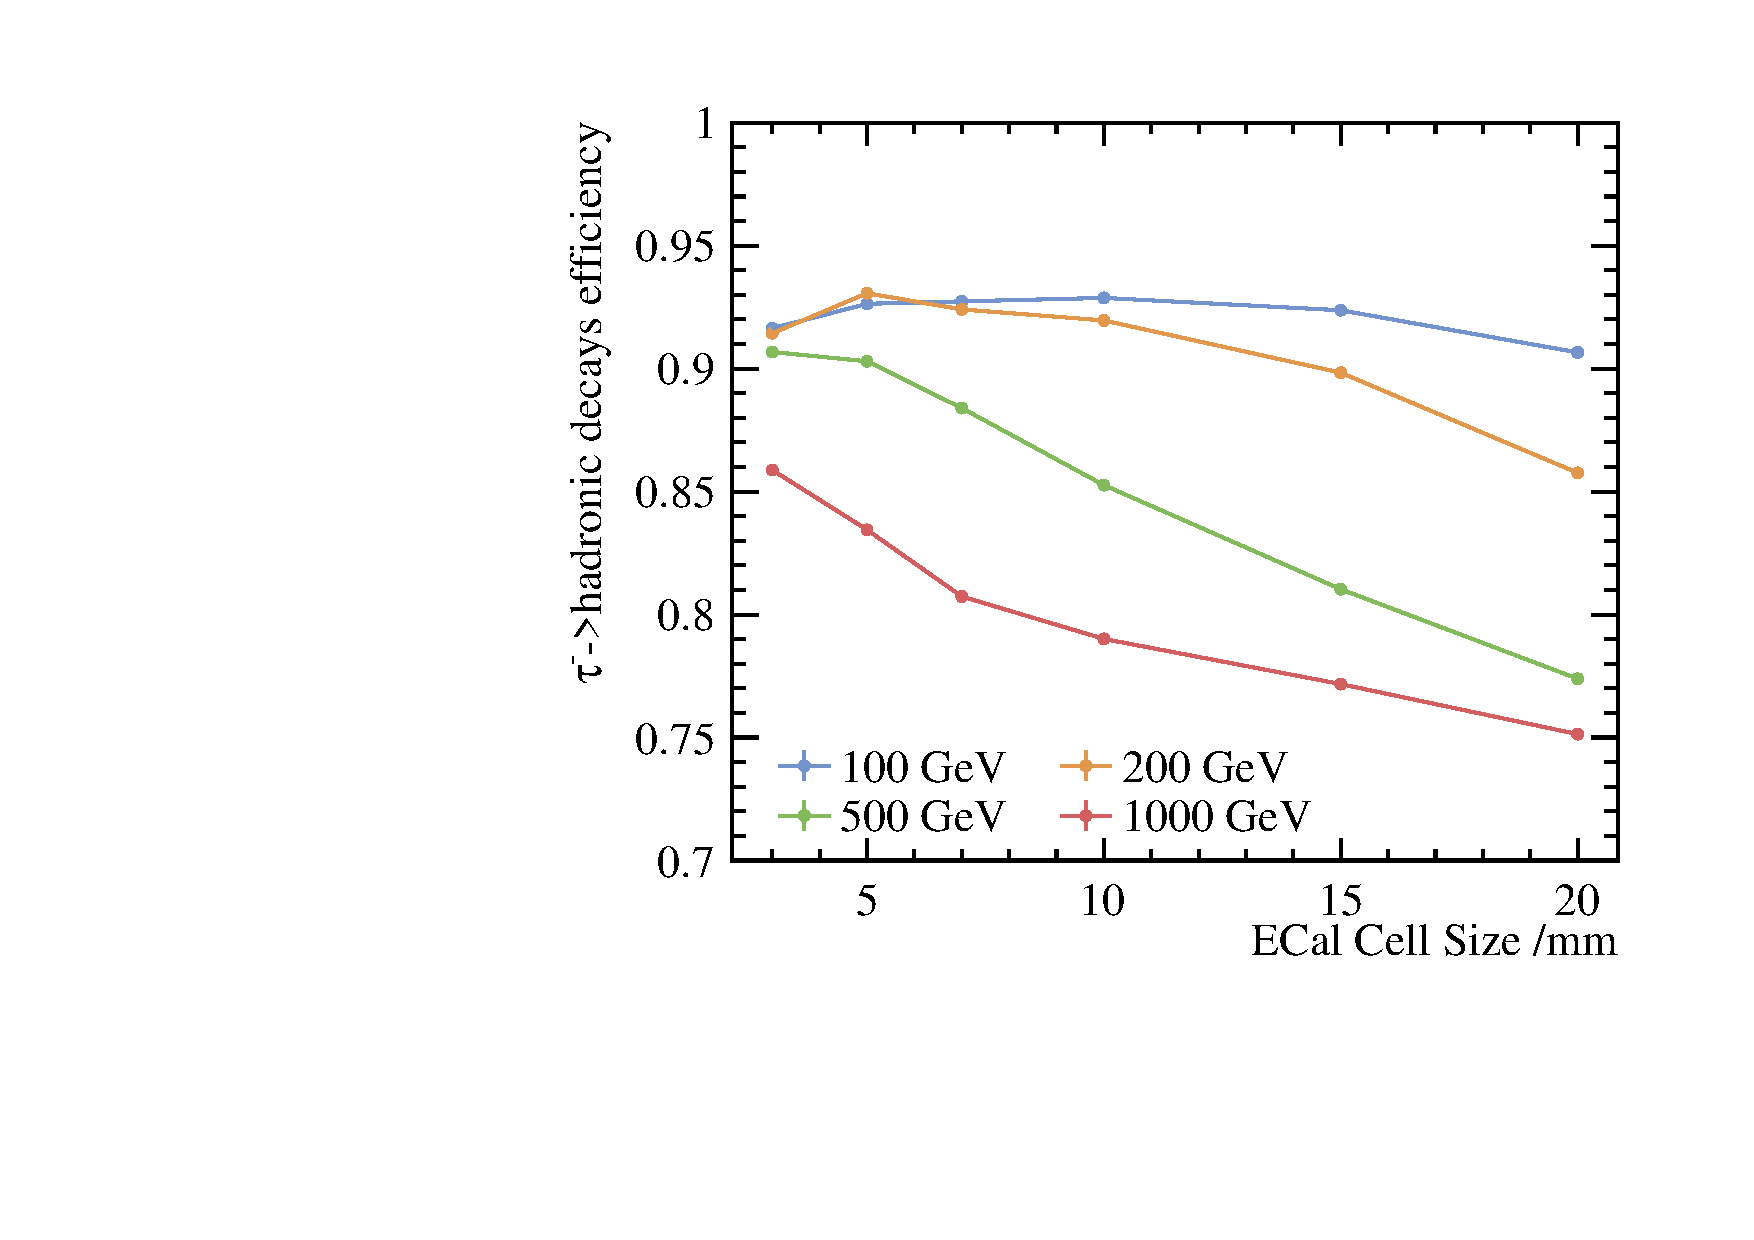
\includegraphics[width=.45\textwidth]{tau/hadronicEff}
% "\includegraphics" from the "graphicx" permits to crop (trim+clip)
% and rotate (angle) and image (and much more)
\caption[]%
{The \Pgt hadronic decay efficiency against the ECal cell size for different \rootS energies with the nominal CLIC\_ILD detector model are shown. The blue, orange, green and red lines are representing the \sqrtS = 100, 200, 500 and 1000\,GeV respectively.}
\label{fig:TauHadronicEfficiency}
\end{figure}


To effectively compare the overall separation power of all hadronic final states across \sqrtS and ECal square cell sizes, we constructed a single parameter function, the  \Pgt hadronic decay final state efficiency function,
\begin{equation}
\label{eq:had}
\tauHad = \frac{\Sigma_{i} {Br}_{i}\varepsilon_{i}}{\Sigma_{i} {Br}_{i}}  \,,
\end{equation}

where $Br_{i}$ is the branching fraction of a hadronic final state after the generator level cut. $\varepsilon_{i}$ is the correct reconstruction efficiency of the final state, and the $i$ is summing over five hadronic decay final state of \Pgt. Leptonic decays, \decayElectron and \decayMuon, were not included, because the variation of the leptonic decay selection efficiency is small.


In the \Figure{fig:TauHadronicEfficiency}, \Pgt hadronic decay final state efficiency, \tauHad, against the ECal cell size with different \sqrtS is shown. \tauHad decreases when cell sizes increases and when \sqrtS increases.  \tauHad of the 5\,mm ECal cell size is better than that of the 3\,mm for \sqrtS = 100 and 200\,GeV lines possibly due the optimisation of the software for the nominal ILD 5\,mm ECal square cell size.

The \tauHad is above 90\% for the ECal cell size from 3 to 20\,mm for the \rootSGeV{100}. For \rootSGeV{200}, the \tauHad decreases from over 90\% to 86\% for the ECal square cell size from 3 to 20\,mm. The degradation of the \tauHad is more significant for the \sqrtS = 500 and 1000\,GeV, where the \tauHad drops from over 90\% to 77\%  and from 86\% to 75\% respectively, over the same range of ECal square cell size.

For \sqrtS = 100 and 200\,GeV, up to 15\,mm cell sizes of ECal will give a good performance for \Pgt hadronic decay modes separation, and the \tauHad is above 90\%. For \sqrtS = 500 and 1000\,GeV, it is preferential to have a small ECal cell size for a good \Pgt hadronic decay modes separation. There is about 15\% degradation of \tauHad for ECal square cell size from 3 to 20\,mm.

\section{} 